\subsection{\vdmh}
\Opensolutionfile{ans}[ans/DA-CD2-VD]
\begin{vd}Tìm các nguyên hàm sau (hàm cơ bản):
 \begin{listEX}[2]
 \item $I= \displaystyle \int (3x^2 + 1) \mathrm{d}x = $\dotfill
 \item $I= \displaystyle \int \frac{1}{x^4} \mathrm{d}x = $\dotfill
 \item $I= \displaystyle \int x\sqrt[3]{x} \mathrm{d}x = $\dotfill
 \item $I= \displaystyle \int \left(\frac{3}{x} - \dfrac{5}{x^2}\right) \mathrm{d}x= $\dotfill
 \item $I = \displaystyle \int (3\cos x - 4\sin x) \mathrm{d}x= $\dotfill
 \item $I= \displaystyle \int \frac{1}{3^x} \mathrm{d}x= $\dotfill
 \item $I= \displaystyle \int \left(\frac{1}{\cos^2 x} - \frac{1}{\sin^2 x}\right) \mathrm{d}x= $\dotfill
 \item $I = \displaystyle \int (2e^x - 5^x) \mathrm{d}x= $\dotfill
 \end{listEX}
\end{vd}
\begin{vd}%[Tự luận - Tích phân]
 Cho hàm số $f(x)$ và $g(x)$ liên tục trên $\mathbb{R}$, thỏa mãn $\int_{1}^{2} f(x)\mathrm{\,d}x = 7$, $\int_{2}^{5} f(x)\mathrm{\,d}x = 4$ và $\int_{1}^{5} g(x)\mathrm{\,d}x = 3$. Tính các tích phân sau
 \begin{listEX}[1]
 \item $I = \int_{1}^{5} f(x) \mathrm{\,d}x=$\dotfill
 \item $I = \int_{1}^{5} \left[ f(x) - 2g(x) \right] \mathrm{\,d}x=$\dotfill
 \item $I = \int_{1}^{5} \left[ 2f(x) - 3x^2 \right] \mathrm{\,d}x=$\dotfill
 \end{listEX}
\end{vd}
\begin{vd}
 Tính $I = \displaystyle\int\limits_{0}^{2} f(x)\mathrm{\,d}x$ biết rằng $f(x)$ liên tục trên $\mathbb{R}$ và $f(x) = \begin{cases} x & \text{khi } -3 \le x < 1 \\ 2x + a & \text{khi } 1 \le x \le 3 \end{cases}$
 \loigiai{
 }
\end{vd}

\begin{vd}
 Tính diện tích và thể tích trong mỗi trường hợp sau:
 \begin{listEX}[2]
 \item $H: \begin{cases} y = x^2 + 3x - 1 \\ Ox \\ x = 1, x = 2 \end{cases} \longrightarrow S_H = \dotfill$
 \item $H: \begin{cases} y = x^2 - 2x \\ y = x \end{cases} \longrightarrow S_H = \dotfill$
 \item $H: \begin{cases} y = x + 1 \\ y = 3x \\ x = 1, x = 3 \end{cases} \longrightarrow V_{Ox} = \dotfill$
 \item $H: \begin{cases} y = 5 - x^2 \\ y = 4x \end{cases} \longrightarrow V_{Ox} = \dotfill$
 \end{listEX}
% \loigiai{
% \textbf{1.} Trục $Ox$ có phương trình $y = 0$.
% Diện tích hình phẳng $H$ cần tính là:
% $$S_H = \int\limits_{1}^{2} \left| x^2 + 3x - 1 \right| \mathrm{\,d}x$$
% Vì $x^2 + 3x - 1 > 0$ với mọi $x \in [1; 2]$ nên ta có thể bỏ dấu giá trị tuyệt đối:
% \begin{eqnarray*}
% S_H &=& \int\limits_{1}^{2} (x^2 + 3x - 1) \mathrm{\,d}x \\
% &=& \left( \dfrac{x^3}{3} + \dfrac{3x^2}{2} - x \right)\Bigg|_1^2 \\
% &=& \left( \dfrac{8}{3} + 6 - 2 \right) - \left( \dfrac{1}{3} + \dfrac{3}{2} - 1 \right) \\
% &=& \dfrac{20}{3} - \dfrac{5}{6} = \dfrac{35}{6}.
% \end{eqnarray*}
% \textbf{Đáp số 1:} $S_H = \dfrac{35}{6}$.
% \textbf{2.} Phương trình hoành độ giao điểm của hai đồ thị:
% $$x^2 - 2x = x \Leftrightarrow x^2 - 3x = 0 \Leftrightarrow \begin{bmatrix} x = 0 \\ x = 3 \end{bmatrix}$$
% Diện tích hình phẳng $H$ là:
% $$S_H = \int\limits_{0}^{3} \left| (x^2 - 2x) - x \right| \mathrm{\,d}x = \int\limits_{0}^{3} \left| x^2 - 3x \right| \mathrm{\,d}x$$
% Trên đoạn $[0; 3]$, biểu thức $x^2 - 3x \le 0$ nên $\left| x^2 - 3x \right| = 3x - x^2$.
% \begin{eqnarray*}
% S_H &=& \int\limits_{0}^{3} (3x - x^2) \mathrm{\,d}x \\
% &=& \left( \dfrac{3x^2}{2} - \dfrac{x^3}{3} \right)\Bigg|_0^3 \\
% &=& \left( \dfrac{27}{2} - \dfrac{27}{3} \right) - 0 = \dfrac{9}{2}.
% \end{eqnarray*}
% \textbf{Đáp số 2:} $S_H = \dfrac{9}{2}$.
% \textbf{3.} Thể tích khối tròn xoay tạo thành khi quay $H$ quanh trục $Ox$ là:
% \begin{eqnarray*}
% V_{Ox} &=& \pi \int\limits_{1}^{3} \left| (3x)^2 - (x+1)^2 \right| \mathrm{\,d}x \\
% &=& \pi \int\limits_{1}^{3} \left| 9x^2 - (x^2 + 2x + 1) \right| \mathrm{\,d}x \\
% &=& \pi \int\limits_{1}^{3} \left| 8x^2 - 2x - 1 \right| \mathrm{\,d}x
% \end{eqnarray*}
% Vì $8x^2 - 2x - 1 > 0$ với mọi $x \in [1; 3]$ nên:
% \begin{eqnarray*}
% V_{Ox} &=& \pi \int\limits_{1}^{3} (8x^2 - 2x - 1) \mathrm{\,d}x \\
% &=& \pi \left( \dfrac{8x^3}{3} - x^2 - x \right)\Bigg|_1^3 \\
% &=& \pi \left[ \left( \dfrac{8 \cdot 27}{3} - 9 - 3 \right) - \left( \dfrac{8}{3} - 1 - 1 \right) \right] \\
% &=& \pi \left( 60 - \dfrac{2}{3} \right) = \dfrac{178\pi}{3}.
% \end{eqnarray*}
% \textbf{Đáp số 3:} $V_{Ox} = \dfrac{178\pi}{3}$.
% \textbf{4.} Phương trình hoành độ giao điểm của hai đồ thị:
% $$5 - x^2 = 4x \Leftrightarrow x^2 + 4x - 5 = 0 \Leftrightarrow \begin{bmatrix} x = 1 \\ x = -5 \end{bmatrix}$$
% Thể tích khối tròn xoay tạo thành khi quay $H$ quanh trục $Ox$ là:
% \begin{eqnarray*}
% V_{Ox} &=& \pi \int\limits_{-5}^{1} \left| (5-x^2)^2 - (4x)^2 \right| \mathrm{\,d}x \\
% &=& \pi \int\limits_{-5}^{1} \left| 25 - 10x^2 + x^4 - 16x^2 \right| \mathrm{\,d}x \\
% &=& \pi \int\limits_{-5}^{1} \left| x^4 - 26x^2 + 25 \right| \mathrm{\,d}x
% \end{eqnarray*}
% Xét dấu biểu thức $f(x) = x^4 - 26x^2 + 25 = (x^2 - 1)(x^2 - 25)$:
% Trên đoạn $[-5; -1]$, ta có $f(x) \le 0$.
% Trên đoạn $[-1; 1]$, ta có $f(x) \ge 0$.
% Do đó, ta tách tích phân:
% $$V_{Ox} = \pi \left( \int\limits_{-5}^{-1} -(x^4 - 26x^2 + 25) \mathrm{\,d}x + \int\limits_{-1}^{1} (x^4 - 26x^2 + 25) \mathrm{\,d}x \right)$$
% Gọi $F(x) = \dfrac{x^5}{5} - \dfrac{26x^3}{3} + 25x$ là một nguyên hàm của $f(x)$. Ta tính:
% $F(-5) = \dfrac{-3125}{5} - \dfrac{26(-125)}{3} - 125 = \dfrac{1000}{3}$.
% $F(-1) = -\dfrac{1}{5} + \dfrac{26}{3} - 25 = -\dfrac{248}{15}$.
% $F(1) = \dfrac{1}{5} - \dfrac{26}{3} + 25 = \dfrac{248}{15}$.
% Thay vào công thức thể tích:
% \begin{eqnarray*}
% V_{Ox} &=& \pi \Big[ -\big( F(-1) - F(-5) \big) + \big( F(1) - F(-1) \big) \Big] \\
% &=& \pi \left[ -\left( -\dfrac{248}{15} - \dfrac{1000}{3} \right) + \left( \dfrac{248}{15} - \left(-\dfrac{248}{15}\right) \right) \right] \\
% &=& \pi \left( \dfrac{5248}{15} + \dfrac{496}{15} \right) = \dfrac{5744\pi}{15}.
% \end{eqnarray*}
% \textbf{Đáp số 4:} $V_{Ox} = \dfrac{5744\pi}{15}$.
% }
\end{vd}
\begin{vd}
 Cho hình phẳng $(H)$ như hình vẽ (phần gạch sọc). Hãy tính diện tích của hình $(H)$ và thể tích khối tròn xoay khi quay hình $(H)$ quanh trục $Ox$
 \begin{listEX}[3]
 \item \includegraphics[width=4cm]{images/2.1}
 \item \includegraphics[width=4cm]{images/2.3}
 \item \includegraphics[width=4cm]{images/2.4}
 \end{listEX}
 \loigiai{
     
 }
\end{vd}
\begin{vd}%[Mức độ 3]%[Chuyên đề Nguyên hàm]
 Cho hàm số $f(x) = 2x + 1$. Gọi $F(x)$ là một nguyên hàm của $f(x)$. Xét tính đúng sai của các khẳng định sau:
 \choiceTF
 {\True $\int f(x)\text{d}x = x^2 + x + C$}
 {$\int \left[ (x - 1) \cdot f(x) \right]\text{d}x = \frac{1}{3}x^3 - x + C$}
 {Nếu $F(1) = 2$ thì $F(x) = x^2 + x - 1$}
 {\True Nếu $F(1) = 2$ và $\frac{1}{F(1)} + \frac{1}{F(2)} + \dots + \frac{1}{F(99)} + \frac{1}{F(100)} = \frac{a}{b}$ thì $a + b = 201$}
 \loigiai{
 \begin{itemize}
 \item Ta có $\int f(x)\text{d}x = \int (2x + 1)\text{d}x = x^2 + x + C$. Do đó khẳng định a đúng.
 \item Ta có $\int \left[ (x - 1) \cdot f(x) \right]\text{d}x = \int (x - 1)(2x + 1)\text{d}x = \int (2x^2 - x - 1)\text{d}x = \frac{2}{3}x^3 - \frac{1}{2}x^2 - x + C$. Khẳng định b sai.
 \item Từ ý a, nguyên hàm $F(x)$ có dạng $F(x) = x^2 + x + C$. 
 Biết $F(1) = 2 \Leftrightarrow 1^2 + 1 + C = 2 \Leftrightarrow C = 0$. 
 Vậy $F(x) = x^2 + x$. Khẳng định c sai. 
 \textit{(Cách khác: Nếu $F(x) = x^2 + x - 1$ thì $F(1) = 1 \neq 2$, do đó có thể kết luận ngay là sai).}
 \item Theo kết quả ý c, ta có $F(x) = x^2 + x = x(x + 1)$.
 Suy ra $\frac{1}{F(n)} = \frac{1}{n(n + 1)} = \frac{1}{n} - \frac{1}{n + 1}$.
 Khi đó tổng:
 \begin{align*}
 S &= \frac{1}{F(1)} + \frac{1}{F(2)} + \dots + \frac{1}{F(100)} \\
 &= \left( 1 - \frac{1}{2} \right) + \left( \frac{1}{2} - \frac{1}{3} \right) + \dots + \left( \frac{1}{100} - \frac{1}{101} \right) \\
 &= 1 - \frac{1}{101} = \frac{100}{101}.
 \end{align*}
 Đồng nhất với $\frac{a}{b}$ (phân số tối giản), ta được $a = 100$ và $b = 101$. 
 Vậy $a + b = 100 + 101 = 201$. Do đó khẳng định d đúng.
 \end{itemize}
 }
 \dotlineEX{2}
\end{vd}
\begin{vd}[MH-BGD-2025] Một người điều khiển ô tô đang ở đường dẫn muốn nhập làn vào đường cao tốc. Khi ô tô cách điểm nhập làn $200 \text{ (m)}$, tốc độ của ô tô là $36 \text{ (km/h)}$. Hai giây sau đó, ô tô bắt đầu tăng tốc với tốc độ $v(t) = at + b$ ($a, b \in \mathbb{R}$, $a > 0$), trong đó $t$ là thời gian tính bằng giây kể từ lúc bắt đầu tăng tốc. Biết rằng ô tô nhập làn cao tốc sau $12$ giây và duy trì sự tăng tốc trong $24$ giây kể từ khi bắt đầu tăng tốc.
\choiceTF
{\True Quãng đường ô tô đi được từ khi bắt đầu tăng tốc đến khi nhập làn là $180 \text{ (m)}$}
{\True Giá trị của $b$ là $10$}
{Quãng đường $S(t)$ (\textit{đơn vị: mét}) mà ô tô đi được trong thời gian $t$ giây ($0 \le t \le 24$) kể từ khi tăng tốc được tính theo công thức $S(t) = \displaystyle\int\limits_{0}^{24} v(t)\mathrm{\,d}t$}
{Sau $24$ giây kể từ khi tăng tốc, tốc độ ô tô không vượt quá tốc độ cho phép $100\text{km/h}$}
 \loigiai{
 Đổi đơn vị: $36 \text{ km/h} = 10 \text{ m/s}$.
 \begin{itemize}
 \item \textbf{Ý a) Đúng.} Trong $2$ giây đầu tiên (trước khi tăng tốc), ô tô chạy với vận tốc không đổi $10 \text{ m/s}$, quãng đường đi được là $s_1 = 10 \cdot 2 = 20 \text{ (m)}$. Khoảng cách còn lại đến điểm nhập làn chính là quãng đường đi được từ lúc bắt đầu tăng tốc đến khi nhập làn: $s_2 = 200 - 20 = 180 \text{ (m)}$.
 \item \textbf{Ý b) Đúng.} Tại thời điểm bắt đầu tăng tốc ($t=0$), vận tốc của ô tô là $10 \text{ m/s}$. Ta có $v(0) = a\cdot 0 + b = 10 \Rightarrow b = 10$.
 \item \textbf{Ý c) Sai.} Quãng đường đi được trong thời gian $t$ giây ($0 \le t \le 24$) kể từ khi tăng tốc phải là tích phân với cận trên là $t$: $S(t) = \displaystyle\int\limits_{0}^{t} v(x)\mathrm{\,d}x$. Viết cận trên là $24$ là sai công thức hàm quãng đường theo thời gian $t$.
 \item \textbf{Ý d) Sai.} Theo ý a) và b), quãng đường đi được trong 12 giây tăng tốc đầu tiên là $180\text{m}$. Hàm vận tốc là $v(t) = at + 10$.
 Ta có: $\displaystyle\int\limits_{0}^{12} (at + 10)\mathrm{\,d}t = 180 \Leftrightarrow \left( \dfrac{at^2}{2} + 10t \right)\Bigg|_0^{12} = 180 \Leftrightarrow 72a + 120 = 180 \Leftrightarrow a = \dfrac{5}{6}$.
 Vậy phương trình vận tốc là $v(t) = \dfrac{5}{6}t + 10$.
 Sau 24 giây, vận tốc của ô tô là: $v(24) = \dfrac{5}{6}\cdot 24 + 10 = 30 \text{ (m/s)}$.
 Đổi sang km/h: $30 \cdot 3{,}6 = 108 \text{ (km/h)}$.
 Vận tốc này đã vượt quá giới hạn $100 \text{ km/h}$, do đó phát biểu là sai.
 \end{itemize}
 }
  \dotlineEX{2}
\end{vd}
\begin{vd}[BGD-2025]%[Mã đề 0102]%[Câu 3]%[MĐ3]
 Đối với ngành nuôi trồng thủy sản, việc kiểm soát lượng thuốc tồn dư trong nước là một nhiệm vụ quan trọng nhằm đáp ứng các tiêu chuẩn an toàn về môi trường. Khi nghiên cứu một loại thuốc trị bệnh trong nuôi trồng thủy sản, người ta sử dụng thuốc đó một lần và theo dõi nồng độ thuốc tồn dư trong nước kể từ lúc sử dụng thuốc. Kết quả cho thấy nồng độ thuốc $y(t)$ (đơn vị: mg/lít) tồn dư trong nước tại thời điểm $t$ ngày ($t \ge 0$) kể từ lúc sử dụng thuốc, thỏa mãn $y(t)>0$ và $y'(t)=k \cdot y(t)$ ($t \ge 0$), trong đó $k$ là hằng số khác không. Đo nồng độ thuốc tồn dư trong nước tại các thời điểm $t=6$ (ngày); $t=12$ (ngày) nhận được kết quả lần lượt là $2$ mg/lít; $1$ mg/lít. Cho biết $y(t)=e^{g(t)}$ ($t \ge 0$).
 \choiceTF
 {\True $g(t)=kt+C$ ($t \ge 0$) với $C$ là một hằng số xác định}
 {\True $k=-\dfrac{\ln 2}{6}$}
 {$C=3 \ln 2$}
 {Nồng độ thuốc tồn dư trong nước tại thời điểm $t=20$ (ngày) kể từ lúc sử dụng thuốc lớn hơn $0,4$ mg/lít}
 \loigiai{
 Từ phương trình $y'(t) = k \cdot y(t) \Rightarrow \dfrac{y'(t)}{y(t)} = k$. \\
 Lấy nguyên hàm hai vế: $\displaystyle\int \dfrac{y'(t)}{y(t)} \text{d}t = \int k \text{d}t \Rightarrow \ln y(t) = kt + C$. \\
 Vì $y(t) = e^{g(t)} \Rightarrow g(t) = \ln y(t)$, do đó $g(t) = kt + C$. Vậy **a) Đúng**. \\
 Ta có hệ phương trình:
 $\begin{cases} g(6) = \ln y(6) \\ g(12) = \ln y(12) \end{cases} \Leftrightarrow \begin{cases} 6k + C = \ln 2 \\ 12k + C = \ln 1 = 0 \end{cases} \Leftrightarrow \begin{cases} 6k = -\ln 2 \\ C = -12k \end{cases} \Leftrightarrow \begin{cases} k = -\dfrac{\ln 2}{6} \\ C = 2\ln 2 \end{cases}$. \\
 Vậy **b) Đúng** và **c) Sai** (vì $C = 2\ln 2$). \\
 Với $t=20$, ta có $g(20) = 20 \cdot \left(-\dfrac{\ln 2}{6}\right) + 2\ln 2 = -\dfrac{10}{3}\ln 2 + 2\ln 2 = -\dfrac{4}{3}\ln 2$. \\
 Nồng độ thuốc: $y(20) = e^{g(20)} = e^{-\frac{4}{3}\ln 2} = 2^{-\frac{4}{3}} \approx 0,3968$ mg/lít. \\
 Vì $0,3968 < 0,4$ nên mệnh đề **d) Sai**.
 }
 \dotlineEX{3}
\end{vd}
\begin{vd}Doanh thu bán hàng $R(x)$của một công ty công nghệ khi bán một loại con chip được cho bởi tốc độ biến đổi doanh thu $M_R(x) = 300 - 0,1x$, trong đó $x$ là số lượng chip đã bán và $M_R(x) = R'(x)$ (triệu đồng). Tìm doanh thu của công ty khi đã bán được $1\,000$ con chip.\shortans{250}
% \loigiai{
%     Hàm doanh thu là một nguyên hàm của hàm tốc độ biến đổi doanh thu:$$R(x) = \int M_R(x) \mathrm{d}x = \int (300 - 0,1x) \mathrm{d}x = 300x - 0,05x^2 + C.$$Giả sử khi chưa bán sản phẩm nào thì doanh thu bằng $0$, tức là $R(0) = 0 \Rightarrow C = 0$. Doanh thu khi bán được $1\,000$ con chip là:$$R(1000) = 300(1000) - 0,05(1000)^2 = 300\,000 - 50\,000 = 250\,000 \text{ (triệu đồng)}.$$Vậy doanh thu của công ty là $250$ tỷ đồng.}
\end{vd}
\begin{vd}
 Một xưởng sản xuất máy công nghiệp đang đưa vào vận hành một dây chuyền tự động mới. Gọi $N(t)$ là tổng số sản phẩm hoàn thiện được sau $t$ tháng áp dụng dây chuyền. Theo đánh giá, tốc độ sản xuất $N'(t)$ (sản phẩm/tháng) của dây chuyền thay đổi theo thời gian và tuân theo công thức $N'(t) = at^2 + bt$ (với $a, b \in \mathbb{R}$). Giả sử tại thời điểm bắt đầu áp dụng, chưa có sản phẩm nào được hoàn thiện. Thống kê cho thấy, sau 2 tháng đầu tiên, dây chuyền sản xuất được $1200$ sản phẩm; sau 4 tháng, tổng số sản phẩm sản xuất được là $8000$. Hỏi sau 5 tháng áp dụng dây chuyền, xưởng đó đã sản xuất được tổng cộng bao nhiêu ngàn sản phẩm?
 \shortans{$15$}
 \loigiai{
 Từ giả thiết, ta có số sản phẩm sản xuất được sau $t$ tháng là nguyên hàm của hàm tốc độ sản xuất:
 $$ N(t) = \int N'(t) \mathrm{\,d}t = \int (at^2 + bt) \mathrm{\,d}t = \dfrac{a}{3}t^3 + \dfrac{b}{2}t^2 + C $$
 Tại thời điểm ban đầu ($t=0$), chưa có sản phẩm nào hoàn thiện nên $N(0) = 0 \Rightarrow C = 0$.
 Do đó, $N(t) = \dfrac{a}{3}t^3 + \dfrac{b}{2}t^2$.
 Theo bài ra, ta có hệ phương trình:
 $$ \begin{cases} N(2) = 1200 \\ N(4) = 8000 \end{cases} \Leftrightarrow \begin{cases} \dfrac{a}{3} \cdot 2^3 + \dfrac{b}{2} \cdot 2^2 = 1200 \\[0.2cm] \dfrac{a}{3} \cdot 4^3 + \dfrac{b}{2} \cdot 4^2 = 8000 \end{cases} \Leftrightarrow \begin{cases} \dfrac{8}{3}a + 2b = 1200 \\[0.2cm] \dfrac{64}{3}a + 8b = 8000 \end{cases} $$
 Quy đồng và rút gọn hệ phương trình trên:
 $$ \begin{cases} 4a + 3b = 1800 \\ 8a + 3b = 3000 \end{cases} $$
 Lấy phương trình dưới trừ phương trình trên ta được $4a = 1200 \Leftrightarrow a = 300$.
 Thay $a=300$ vào phương trình đầu: $4(300) + 3b = 1800 \Leftrightarrow 1200 + 3b = 1800 \Leftrightarrow 3b = 600 \Leftrightarrow b = 200$.
 Vậy hàm số biểu diễn tổng số sản phẩm là:
 $$ N(t) = \dfrac{300}{3}t^3 + \dfrac{200}{2}t^2 = 100t^3 + 100t^2 $$
 Số sản phẩm sản xuất được tổng cộng sau 5 tháng là:
 $$ N(5) = 100 \cdot 5^3 + 100 \cdot 5^2 = 100 \cdot 125 + 100 \cdot 25 = 12500 + 2500 = 15000 \text{ (sản phẩm)}. $$
 }
 \dotlineEX{1}% Tạo các dòng kẻ trong tài liệu
\end{vd}
\begin{vd}
 \immini[thm]{ Một xe ô tô sau khi chờ hết đèn đỏ đã bắt đầu chuyển động với vận tốc được biểu thị bằng đồ thị là đường cong parabol. Biết rằng sau $5$ phút thì xe đạt đến vận tốc cao nhất $1000$ mét/phút và bắt đầu giảm tốc, đi được $6$ phút thì xe chuyển động đều. Quãng đường xe đi được sau $10$ phút đầu tiên kể từ khi hết đèn đỏ là bao nhiêu mét?
 \shortans{8160}}{\begin{tikzpicture}[>=stealth, yscale=.5,xscale=0.5]
     \draw[->] (-1,0) -- (13,0) node[below] {$t (\text{phút})$};
     \draw[->] (0,-1) -- (0,5) node[right] {$v (\text{mét/phút})$};
     \node at (0,0) [below left] {$O$};
     \draw[blue] plot[domain=0:6, samples=100] (\x, {-40*(\x)^2/250 + 400*(\x)/250});
     \draw[blue] (6, 3.84) -- (10, 3.84);
     \draw[dashed] (5,0) node[below] {$5$} -- (5,4) -- (0,4) node[left] {$1000$};
     \draw[dashed] (6,0) node[below] {$6$} -- (6,3.84);
     \draw[dashed] (10,0) node[below] {$10$} -- (10,3.84);
     \end{tikzpicture}}
% \loigiai{
% Gọi phương trình vận tốc của xe ô tô trên đoạn $[0; 6]$ (đường parabol) là $v_1(t) = at^2 + bt + c$ $(a \neq 0)$.
% Từ đồ thị, ta thấy parabol đi qua gốc tọa độ $O(0;0)$ nên $c = 0$.
% Parabol có đỉnh tại $t = 5$, $v = 1000$ nên ta có hệ phương trình:
% $$\begin{cases} -\dfrac{b}{2a} = 5 \\ a\cdot 5^2 + b\cdot 5 = 1000 \end{cases} \Leftrightarrow \begin{cases} b = -10a \\ 25a - 50a = 1000 \end{cases} \Leftrightarrow \begin{cases} b = 400 \\ a = -40 \end{cases}$$
% Suy ra phương trình vận tốc trên $[0; 6]$ là $v_1(t) = -40t^2 + 400t$.
% Tại thời điểm $t = 6$ phút, vận tốc của xe là:
% $$v_1(6) = -40\cdot 6^2 + 400\cdot 6 = 960 \text{ (mét/phút)}$$
% Từ thời điểm $t = 6$ đến $t = 10$, xe chuyển động đều nên phương trình vận tốc là $v_2(t) = 960$.
% Quãng đường xe đi được sau $10$ phút đầu tiên là:
% \begin{eqnarray*}
% S &=& \int\limits_{0}^{6} v_1(t)\mathrm{\,d}t + \int\limits_{6}^{10} v_2(t)\mathrm{\,d}t \\
% &=& \int\limits_{0}^{6} (-40t^2 + 400t)\mathrm{\,d}t + \int\limits_{6}^{10} 960\mathrm{\,d}t \\
% &=& \left( -\dfrac{40}{3}t^3 + 200t^2 \right)\Bigg|_0^6 + \big( 960t \big)\Bigg|_6^{10} \\
% &=& \left( -\dfrac{40}{3}\cdot 6^3 + 200\cdot 6^2 \right) + 960(10 - 6) \\
% &=& 4320 + 3840 = 8160 \text{ (m)}.
% \end{eqnarray*}
% \textbf{Đáp số:} $S = 8160 \text{ (m)}$.
% }
\end{vd}
\begin{vd}
 \immini[thm]{ Một công ty quảng cáo $X$ muốn làm một bức tranh trang trí hình $MNEIF$ ở chính giữa của một bức tường hình chữ nhật $ABCD$ có chiều cao $BC = 6\text{m}$, chiều dài $CD = 12\text{m}$. Cho biết $MNEF$ là hình chữ nhật có $MN = 4\text{m}$; cung $EIF$ có hình dạng là một phần của cung parabol có đỉnh $I$ là trung điểm của cạnh $AB$ và đi qua hai điểm $C, D$. Kinh phí làm bức tranh là $900.000 \text{ đồng/m}^2$. Hỏi công ty $X$ cần bao nhiêu triệu đồng tiền để làm bức tranh đó? (làm tròn kết quả đến hàng phần chục).
 \shortans{20,8}}{ \includegraphics[scale=.3]{images/2.5}}
 \loigiai{
 Chọn hệ trục tọa độ $Oxy$ với gốc $O$ là trung điểm của đoạn $CD$. Trục $Ox$ nằm trên $CD$.
 Khi đó ta có các tọa độ: $C(6; 0)$, $D(-6; 0)$, $I(0; 6)$.
 Giả sử phương trình parabol là $y = ax^2 + 6$. Vì đi qua $C(6; 0)$ nên: $a\cdot 6^2 + 6 = 0 \Leftrightarrow a = -\dfrac{1}{6}$.
 Phương trình parabol là: $y = -\dfrac{1}{6}x^2 + 6$.
 Vùng bức tranh giới hạn bởi hoành độ từ $x_M = -2$ đến $x_N = 2$.
 Diện tích bức tranh là:
 $$S = \int\limits_{-2}^{2} \left( -\dfrac{1}{6}x^2 + 6 \right)\mathrm{\,d}x = 2 \left( -\dfrac{x^3}{18} + 6x \right)\Bigg|_0^2 = 2\left( -\dfrac{8}{18} + 12 \right) = \dfrac{208}{9} \text{ (m}^2\text{)}.$$
 Số tiền cần để làm bức tranh là:
 $$T = \dfrac{208}{9} \times 0{,}9 = 20{,}8 \text{ (triệu đồng)}.$$
 }
\end{vd}
\begin{vd}
 \immini[thm]{ Một thùng nước có dạng hình tròn xoay với đường sinh là một cung của đường tròn,hai đáy là hai hình tròn bằng nhau và có đường kính bằng $20\text{ cm}$, khoảng cách giữa hai đáy bằng $32\text{ cm}$, đường kính lớn nhất của thân thùng là $24\text{ cm}$ (biết các kích thước đã trừ lớp vỏ thùng, tham khảo hình vẽ). Hỏi phần không gian bên trong thùng có thể tích bằng bao nhiêu lít? (Kết quả lấy đến chữ số hàng phần chục và không làm tròn).
 \shortans{12,9}}{\includegraphics[scale=.3]{images/2.8}}
 \loigiai{
 Chọn hệ trục tọa độ $Oxy$ sao cho trục $Ox$ trùng với trục của thùng rượu, gốc tọa độ $O$ là tâm đối xứng của thùng.
 \begin{itemize}
 \item Vì khoảng cách giữa hai đáy là $32\text{ cm}$ nên giới hạn của hình phẳng dọc theo trục $Ox$ là từ $x = -16$ đến $x = 16$.
 \item Đường kính đáy bằng $20\text{ cm} \Rightarrow$ bán kính đáy $r = 10\text{ cm}$. Điểm tương ứng trên cung tròn là $M(16; 10)$.
 \item Đường kính lớn nhất bằng $24\text{ cm} \Rightarrow$ bán kính lớn nhất tại tâm $R_{max} = 12\text{ cm}$. Điểm tương ứng trên cung tròn là $A(0; 12)$.
 \end{itemize}
 Gọi phương trình đường tròn chứa cung tròn là $x^2 + (y - k)^2 = R^2$ (với tâm $I(0; k)$ nằm trên trục $Oy$).\\
 Do đường tròn đi qua $A(0; 12)$ và $M(16; 10)$ nên ta có:
 $$ \begin{cases} 0^2 + (12 - k)^2 = R^2 \\ 16^2 + (10 - k)^2 = R^2 \end{cases} \Rightarrow (12 - k)^2 = 256 + (10 - k)^2 $$
 $$ \Leftrightarrow 144 - 24k + k^2 = 256 + 100 - 20k + k^2 \Leftrightarrow -4k = 212 \Leftrightarrow k = -53. $$
 Khi đó $R^2 = (12 - (-53))^2 = 65^2 = 4225$.
 Phương trình cung tròn (phần $y > 0$) là: $y = \sqrt{4225 - x^2} - 53$.
 Thể tích của thùng rượu là vật thể tròn xoay khi quay quanh trục $Ox$:
 $$ V = \pi \int_{-16}^{16} \left( \sqrt{4225 - x^2} - 53 \right)^2 \text{d}x $$
 Sử dụng máy tính cầm tay tính giá trị tích phân:
 $$ V \approx 12983,33 \text{ cm}^3 \approx 12,9833 \text{ lít}. $$
 Theo yêu cầu "lấy đến chữ số hàng phần chục và không làm tròn", ta lấy chữ số đầu tiên sau dấu phẩy mà không tăng đơn vị:
 $$ V = 12,9 \text{ lít}. $$
 \textbf{Đáp số:} $12,9$ lít.
 }
\end{vd}
\begin{vd}[BGD-2025]
    Để đặt được một vật trang trí trên mặt bàn, người ta thiết kế một chân đế như sau. Lấy một khối gỗ có dạng khối chóp cụt tứ giác đều với độ dài hai cạnh đáy lần lượt bằng $7{,}4$ cm và $10{,}4$ cm, bề dày của khối gỗ bằng $1{,}5$ cm. Sau đó khoét bỏ đi một phần của khối gỗ sao cho phần đó có dạng vật thể $H$, ở đó $H$ nhận được bằng cách cắt khối cầu bán kính $5{,}8$ cm bởi một mặt phẳng cắt mà mặt cắt là hình tròn bán kính $3{,}5$ cm (xem hình dưới).\\
    \centerline{
        \begin{tikzpicture}[line join=round, line cap=round,>=stealth,thick,scale=.7]
            % Hình trái
            \coordinate (A) at (0,0);
            \coordinate (B) at (-1.5,-1);
            \coordinate (D) at (4,0);
            \coordinate (C) at ($(B)+(D)-(A)$);
            \coordinate (O) at ($(A)!0.5!(C)$);
            \coordinate (I) at ($(O)+(0,3.5)$);
            \coordinate (A') at ([scale around={0.71:(I)}] A);
            \coordinate (B') at ([scale around={0.71:(I)}] B);
            \coordinate (C') at ([scale around={0.71:(I)}] C);
            \coordinate (D') at ([scale around={0.71:(I)}] D);
            \coordinate (O') at ($(A')!0.5!(C')$);
            \draw(B)--(C)--(D)--(D')--(C')--(B')--(A')--(D') (C)--(C') (B)--(B');
            \draw[dashed,thin](A')--(A)--(B) (A)--(D);
            \draw[dashed,<->](O)--(O')node[right,pos=0.3]{\tiny $1{,}5$ cm};
            \coordinate (vt) at (0,0.2);
            \coordinate (A1) at ($(A')+(vt)$);
            \coordinate (D1) at ($(D')+(vt)$);
            \draw[|<->|](A1)--(D1)node[above,sloped,pos=0.5]{\tiny $7{,}4$ cm};
            \coordinate (vt1) at (0,0.1);
            \coordinate (B1) at ($(B)-(vt)$);
            \coordinate (C1) at ($(C)-(vt)$);
            \draw[|<->|](B1)--(C1)node[below,sloped,pos=0.5]{\tiny $10{,}4$ cm};
        \end{tikzpicture}\qquad
        \begin{tikzpicture}[line join=round, line cap=round,>=stealth,thick,scale=0.5]
            % Hình giữa
            \def\bk{3}
            \def\bkba{0.15}
            \def\bkbb{0.8}
            \def\ga{-50}
            \def\gb{180-\ga}
            \def\gc{0-\gb}
            \coordinate (O) at (0,0);
            \coordinate (M) at ($(O) + (\ga:\bk)$);
            \coordinate (N) at ($(O) + (\gb:\bk)$);
            \coordinate (I) at ($(M)!0.5!(N)$);
            \draw[name path=c1,dashed] (M) arc (\ga:\gb:\bk);
            \path let \p1=(I),\p2=(M),\n1={scalar(veclen(\x2-\x1,\y2-\y1)/1cm)} in \pgfextra{\xdef\bke{\n1}};
            \fill[gray](M) arc (\ga:\gc:\bk)--(N) arc (180:0:\bke cm and \bkba cm)--cycle;
            \draw[name path=c1] (M) arc (\ga:\gc:\bk);
            \draw[name path=ne1,dashed] (M) arc (0:180:\bke cm and \bkba cm) (M)--(N);
            \draw[name path=ne1] (M) arc (0:-180:\bke cm and \bkba cm);
            \draw[name path=ela,dashed] (O) ellipse (\bk cm and \bkbb cm) ($(O)-(\bk,0)$)--($(O)+(\bk,0)$);
            \coordinate (P) at ($(O) + (250:0.9*\bk)$);
            \coordinate (Q) at ($(O) + (235:1.1*\bk)$);
            \path(Q) node [left] {\Large\bf $H$};
            \draw[->](Q)--(P);
        \end{tikzpicture}\qquad
        \begin{tikzpicture}[line join=round, line cap=round,>=stealth,thick,rotate=90,scale=0.5]
            % Hình phải
            \def\bk{3}
            \def\bkba{0.15}
            \def\bkbb{0.8}
            \def\ga{-50}
            \def\gb{180-\ga}
            \def\gc{0-\gb}
            \coordinate (O) at (0,0);
            \coordinate (M) at ($(O) + (\ga:\bk)$);
            \coordinate (N) at ($(O) + (\gb:\bk)$);
            \coordinate (I) at ($(M)!0.5!(N)$);
            \coordinate (J) at ($(O)+(M)-(I)$);
            \draw(M) arc (\ga:\gb:\bk);
            \path let \p1=(I),\p2=(M),\n1={scalar(veclen(\x2-\x1,\y2-\y1)/1cm)} in \pgfextra{\xdef\bke{\n1}};
            \fill[gray](M) arc (\ga:-90:\bk)--(I)--cycle;
            \draw(M) arc (\ga:\gc:\bk);
            \draw(M) arc (0:180:\bke cm and \bkba cm);
            \draw[dashed](M) arc (0:-180:\bke cm and \bkba cm);
            \coordinate (P) at ($(O) + (250:0.9*\bk)$);
            \coordinate (Q) at ($(O) + (235:1.1*\bk)$);
            \path(Q) node [below] {\Large\bf $H$};
            \coordinate (A) at ($(O) + (180:\bk)$);
            \coordinate (B) at ($(O) + (0:\bk)$);
            \coordinate (C) at ($(O) + (-90:\bk)$);
            \coordinate (D) at ($(O) + (90:\bk)$);
            \draw(B) arc (0:180:\bk cm and \bkbb cm);
            \draw[dashed](B) arc (0:-180:\bk cm and \bkbb cm);
            \draw[dashed](J)--(M)--(N) (C)--(D) (A)--(B);
            \draw[->](Q)--(P);
            \draw[->](C)--($(C)-(0,0.5)$)node[below]{$x$};
            \draw[->](B)--($(B)+(0.5,0)$)node[right]{$y$};
            \draw(A)--($(A)-(0.5,0)$) (D)--($(D)+(0,0.5)$); 
            \path(O) node[below left]{$O$};
            \path(J) node[left=-0.05]{\tiny $3{,}5$};
            \path($(B)+(0.15,0)$)node[left]{\tiny $5{,}8$};
        \end{tikzpicture}
    }\\
    Thể tích của khối chân đế bằng bao nhiêu centimét khối (không làm tròn kết quả các phép tính trung gian, chỉ làm tròn kết quả cuối cùng đến hàng phần mười)?
    \shortans{$96{,}5$}
    \loigiai{
        Gọi $V_2$ là thể tích khối chóp cụt, $V_1$ là thể tích khối chỏm cầu.\\
        Ta có 
        \begin{itemize}
            \item 	Diện tích đáy lớn là $10{,}4^2 = 108{,}16$ cm$^2$.
            \item  Diện tích đáy nhỏ là $7{,}4^2 = 54{,}76$ cm$^2$.
            \item  	Chiều cao là $1{,}5$ cm.
        \end{itemize}
        Thể tích của khối chóp cụt là $V_2 = \dfrac{1{,}5}{3} \left(108{,}16 + 54{,}76 + \sqrt{108{,}16 \cdot 54{,}76} \right) =119{,}94$ cm$^3$.\\
        Phương trình đường tròn $(C)$ tâm $O$, bán kính $R = 5{,}8$ là
        $$(C)\colon x^2 + y^2 = 5{,}8^2 \Rightarrow y = \sqrt{5{,}8^2 - x^2} \quad \text{(nửa đường tròn trên).}$$
        Hoành độ giao điểm của hình tròn bán kính $3{,}5$ trong hình và  $(C)$ là
        $$\sqrt{5{,}8^2 - x^2} = 3{,}5 \Rightarrow x^2 =\dfrac{2139}{100} \Rightarrow x = \dfrac{\sqrt{2139}}{10}.$$
        Thể tích của khối chỏm cầu là 
        $$V_1 = \pi\displaystyle \int\limits_{\tfrac{\sqrt{2139}}{10}}^{5{,}8} \left(5{,}8^2 - x^2 \right)\mathrm{\,d}x.$$
        Vậy thể tích của khối chân đế là $V= V_2 - V_1 \approx 96{,}5$ cm$^3$.
    }
    \end{vd}
\begin{vd}
 \immini[thm]{ Từ một khúc gỗ hình trụ có đường kính $30\text{ cm}$, người ta cắt khúc gỗ bởi một mặt phẳng đi qua đường kính đáy và nghiêng với đáy một góc $45^\circ$ để lấy một hình nêm. Kí hiệu $V$ là thể tích của hình nêm. Tính $V (\text{cm}^3)$.
 \shortans{2250}
 }{
 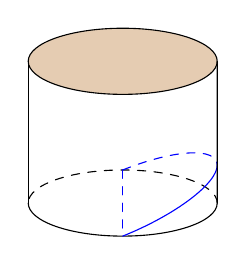
\begin{tikzpicture}[line join=round, line cap=round,>=stealth,scale=0.6]
    \def\a{2}
    \def\b{.7}
    \def\h{3}
    \coordinate (O) at (0,0);
    \coordinate (A) at (\a,0);
    \coordinate (B) at (0,\b);
    \coordinate (O') at (0,\h);
    \draw[fill=brown!40] (O') ellipse (\a cm and \b cm);
    \draw[dashed] (A) arc(0:180:{\a} and {\b});
    \draw (A) arc(0:-180:{\a} and {\b});
    \draw[blue,yslant=.4,dashed] (B) arc(90:0:{\a} and {\b}) coordinate (C);
    \draw[blue,yslant=.4] (0,-\b) arc (-90:0:{\a} and {\b});
    \draw [dashed,blue] (B)--(0,-\b); ;\draw (A)--(\a,\h);\draw (-\a,0)--(-\a,\h);
\end{tikzpicture}
 }
% \loigiai{
% Bán kính đường tròn đáy là $R = 15\text{ cm}$.
% Chọn hệ trục tọa độ sao cho mặt đáy hình nêm nằm trên mặt phẳng $Oxy$, giới hạn bởi nửa đường tròn $x^2 + y^2 = R^2$ ($y \ge 0$) và trục hoành $Ox$ là giao tuyến của mặt phẳng cắt và mặt đáy.
% Mặt phẳng vuông góc với trục $Ox$ tại điểm có hoành độ $x$ (với $x \in [-R; R]$) cắt hình nêm theo thiết diện là một tam giác vuông.
% Độ dài đáy tam giác là $y = \sqrt{R^2 - x^2}$. Do góc nghiêng là $45^\circ$, chiều cao tam giác cũng là $y = \sqrt{R^2 - x^2}$.
% Diện tích thiết diện là:
% $$S(x) = \dfrac{1}{2}y \cdot y = \dfrac{1}{2}y^2 = \dfrac{1}{2}(R^2 - x^2)$$
% Thể tích hình nêm là:
% $$V = \int\limits_{-R}^{R} S(x)\mathrm{\,d}x = 2\int\limits_{0}^{R} \dfrac{1}{2}(R^2 - x^2)\mathrm{\,d}x = \left( R^2x - \dfrac{x^3}{3} \right)\Bigg|_0^R = \dfrac{2}{3}R^3.$$
% Thay $R = 15$, ta được $V = \dfrac{2}{3} \cdot 15^3 = 2250 \text{ (cm}^3\text{)}.$
% }
\dotlineEX{2}
\end{vd}
\begin{vd}
 \immini[thm]{ Một bồn hình trụ đang chứa dầu,được đặt nằm ngang,có chiều dài bồn là $5\text{m}$, có bán kính đáy $1\text{m}$. Người ta đã rút dầu trong bồn tương ứng với $0{,}5\text{m}$ của đường kính đáy. Tính thể tích của lượng dầu còn lại trong bồn theo đơn vị $\text{m}^3$ (làm tròn đến hàng phần chục).
 \shortans{12,6}
 }{\includegraphics[scale=.2]{images/2.7}}
% \loigiai{
% Chọn hệ trục tọa độ với gốc tọa độ tại tâm của mặt đáy. Bán kính đường tròn đáy là $R = 1$.
% Mức dầu còn lại tương ứng với $x \in [-1; 0{,}5]$.
% Thiết diện cắt vuông góc với trục $Ox$ tại điểm có hoành độ $x$ là một hình chữ nhật $ABCD$ có chiều dài bằng chiều dài bồn ($5\text{m}$) và chiều rộng là $AB = 2\sqrt{1 - x^2}$.
% Diện tích thiết diện là: $S(x) = 5 \cdot 2\sqrt{1 - x^2} = 10\sqrt{1 - x^2}$.
% Thể tích lượng dầu còn lại trong bồn là:
% $$V = \int\limits_{-1}^{0{,}5} 10\sqrt{1 - x^2}\mathrm{\,d}x \approx 12{,}6 \text{ (m}^3\text{)}.$$
% }
\dotlineEX{2}
\end{vd}
\Closesolutionfile{ans}
\subsection{\btrl}
\Opensolutionfile{ans}[ans/DA-CD2-BTRL]
\begin{ex}[BGD-2025]%[Câu 4]
 Họ nguyên hàm của hàm số $f(x) = \sin x + \cos x$ là
 \choice
 {$\cos x + \sin x + C$}
 {$\cos x - \sin x + C$}
 {$-\cos x - \sin x + C$}
 {\True $-\cos x + \sin x + C$}
% \loigiai{
% Ta có $\displaystyle\int (\sin x + \cos x) \,\text{d}x = \int \sin x \,\text{d}x + \int \cos x \,\text{d}x = -\cos x + \sin x + C$.
% }
\end{ex}
\begin{ex}[MH BGD-2025]%[Câu 1]
 Nguyên hàm của hàm số $f(x) = e^x$ là:
 \choice
 {$\dfrac{e^{x+1}}{x+1} + C$}
 {\True $e^x + C$}
 {$\dfrac{e^x}{x} + C$}
 {$x.e^{x-1} + C$}
% \loigiai{
% Theo bảng nguyên hàm các hàm số cơ bản: $\displaystyle\int e^x \,\text{d}x = e^x + C$.
% }
\end{ex}
% --- MỨC ĐỘ 1: CÔNG THỨC NGUYÊN HÀM CƠ BẢN ---
\begin{ex}
 [ĐH Vinh-2025] Nguyên hàm của hàm số $f(x) = x - \sin x$ là
 \choice
 {\True $\frac{x^2}{2} + \cos x + C$}
 {$x^2 - \cos x + C$}
 {$\frac{x^2}{2} - \cos x + C$}
 {$2x^2 + \cos x + C$}
% \loigiai{
% Ta có $\int f(x)\mathrm{d}x = \int (x - \sin x)\mathrm{d}x = \frac{x^2}{2} - (-\cos x) + C = \frac{x^2}{2} + \cos x + C$.
% }
\end{ex}
\begin{ex}[KHTN-Hà Nội-2025]
 Họ nguyên hàm của hàm số $f(x) = x + \mathrm{e}^{2x}$ là
 \choice
 {\True $\frac{x^2 + \mathrm{e}^{2x}}{2} + C$}
 {$\frac{x^2 + \mathrm{e}^x}{2} + C$}
 {$\frac{x^2}{2} + \frac{\mathrm{e}^{2x+1}}{2x+1} + C$}
 {$\frac{x^2}{2} + 2\mathrm{e}^{2x} + C$}
% \loigiai{
% Ta có $\int \left(x + \mathrm{e}^{2x}\right)\mathrm{d}x = \frac{x^2}{2} + \frac{1}{2}\mathrm{e}^{2x} + C = \frac{x^2 + \mathrm{e}^{2x}}{2} + C$.
% }
\end{ex}
\begin{ex}[THPT Lương Thế Vinh - Hà Nội - 2025]
Họ các nguyên hàm của hàm số $f(x) = 6x^2 - \sin 2x$.
 \choice
 {$2x^3 + \cos 2x + C$}
 {\True $2x^3 + \frac{1}{2}\cos 2x + C$}
 {$2x^3 - \frac{1}{2}\cos 2x + C$}
 {$3x^2 + \frac{1}{2}\cos 2x + C$}
% \loigiai{
% Ta có $\int \left(6x^2 - \sin 2x\right)\mathrm{d}x = 6\cdot\frac{x^3}{3} - \left(-\frac{1}{2}\cos 2x\right) + C = 2x^3 + \frac{1}{2}\cos 2x + C$.
% }
\end{ex}
\begin{ex}%[2D4N1-3]
    Mệnh đề nào {\bf sai} trong các mệnh đề sau?
    \choice
    {$\displaystyle\int\cos x\mathrm{\,d}x=\sin x+C$}
    {$\displaystyle\int \dfrac{1}{\sin^2x}\mathrm{\,d}x=-\cot x+C$}
    {$\displaystyle\int \dfrac{1}{\cos^2x} \mathrm{\,d}x=\tan x+C$}
    {\True $\displaystyle\int \sin x\mathrm{\,d}x=\cos x+C$}
%    \loigiai{
%        Mệnh đề sai là $\displaystyle\int \sin x\mathrm{\,d}x=\cos x+C$.
%    }
\end{ex}
\begin{ex}[Liên Trường THPT-Nghệ An-2025]
Cho hàm số $f(x) = 3^x + \sin x$. Một nguyên hàm của $f(x)$ trên $\mathbb{R}$ là
 \choice
 {$F(x) = 3^x \ln 3 + \cos x$}
 {$F(x) = 3^x + \sin x$}
 {\True $F(x) = \frac{3^x}{\ln 3} - \cos x$}
 {$F(x) = \frac{3^x}{\ln 3} - \sin x$}
% \loigiai{
% Ta có họ nguyên hàm của $f(x)$ là $\int \left(3^x + \sin x\right)\mathrm{d}x = \frac{3^x}{\ln 3} - \cos x + C$. 
% Chọn $C=0$, ta được một nguyên hàm là $F(x) = \frac{3^x}{\ln 3} - \cos x$.
% }
\end{ex}
\begin{ex}%[734734]%[MĐ1]
 Hàm số $f(x)$ có một nguyên hàm là hàm số $g(x)$ trên khoảng $K$ nếu
 \choice
 {$g'(x)=f(x)+C, \forall x \in K$}
 {\True $g'(x)=f(x), \forall x \in K$}
 {$g(x)=f(x), \forall x \in K$}
 {$f'(x)=g(x), \forall x \in K$}
% \loigiai{
% Theo định nghĩa: Hàm số $g(x)$ được gọi là nguyên hàm của hàm số $f(x)$ trên $K$ nếu $g'(x) = f(x)$ với mọi $x \in K$.
% }
\end{ex}
\begin{ex}%[147850]%[MĐ1]
 Mệnh đề nào dưới đây là sai?
 \choice
 {$\displaystyle\int [f(x)+g(x)]\,\text{d}x=\int f(x)\,\text{d}x+\int g(x)\,\text{d}x$, với mọi hàm $f(x), g(x)$ liên tục trên $\mathbb{R}$}
 {$\displaystyle\int [f(x)-g(x)]\,\text{d}x=\int f(x)\,\text{d}x-\int g(x)\,\text{d}x$, với mọi hàm $f(x), g(x)$ liên tục trên $\mathbb{R}$}
 {\True $\displaystyle\int kf(x)\,\text{d}x=k\int f(x)\,\text{d}x$, với mọi hằng số $k$ và với mọi hàm $f(x)$ liên tục trên $\mathbb{R}$}
 {$\displaystyle\int f'(x)\,\text{d}x=f(x)+C$, với mọi hàm $f(x)$ có đạo hàm trên $\mathbb{R}$}
% \loigiai{
% Theo tính chất của nguyên hàm, tính chất $\displaystyle\int kf(x)\,\text{d}x = k\displaystyle\int f(x)\,\text{d}x$ chỉ khẳng định đúng với mọi hằng số $k \neq 0$.
% }
\end{ex}
\begin{ex}%[360251]%[MĐ1]%[SGK Cánh Diều]
 Hàm số $F(x)=x^3+5$ là nguyên hàm của hàm số:
 \choice
 {\True $f(x)=3x^2$}
 {$f(x)=\dfrac{x^4}{4}+5x+C$}
 {$f(x)=\dfrac{x^4}{4}+5x$}
 {$f(x)=3x^2+5$}
% \loigiai{
% Ta có $f(x) = F'(x) = (x^3+5)' = 3x^2$.
% }
\end{ex}
\begin{ex}%[2D4H1-4]
    Họ nguyên hàm của hàm số $f(x)= \mathrm{e}^x \left(1- \dfrac{2\mathrm{e}^{-x}}{x^3} \right)$ là
    \choice
    {\True $\dfrac{1}{x^2}+\mathrm{e}^x+C$}
    {$\dfrac{2}{x^2}+\mathrm{e}^x+C$}
    {$\dfrac{2}{x^4}+\mathrm{e}^x+C$}
    {$\dfrac{1}{x^4}+\mathrm{e}^x+C$}
%    \loigiai{
%        Ta có $f(x)= \mathrm{e}^x \left(1- \dfrac{2\mathrm{e}^{-x}}{x^3} \right)= \mathrm{e}^x- \dfrac{2}{x^3}$.\\
%        Do đó $\displaystyle \int f(x) \mathrm{\,d}x= \displaystyle \int \left(\mathrm{e}^x- \dfrac{2}{x^3}\right) \mathrm{\,d}x=\dfrac{1}{x^2}+\mathrm{e}^x+C$.
%    }
    \dotlineEX{1}% Tạo các dòng kẻ trong tài liệu
\end{ex}
\begin{ex}%[148297]%[MĐ2]
 Tìm họ nguyên hàm của hàm số $f(x)=\dfrac{2x^2+x-1}{x^2}$.
 \choice
 {$\displaystyle\int \dfrac{2x^2+x-1}{x^2}\,\text{d}x = 2 + \dfrac{1}{x} - \dfrac{1}{x^2} + C$}
 {\True $\displaystyle\int \dfrac{2x^2+x-1}{x^2}\,\text{d}x = 2x + \dfrac{1}{x} + \ln|x| + C$}
 {$\displaystyle\int \dfrac{2x^2+x-1}{x^2}\,\text{d}x = x^2 + \dfrac{1}{x} + \ln|x| + C$}
 {$\displaystyle\int \dfrac{2x^2+x-1}{x^2}\,\text{d}x = x^2 - \dfrac{1}{x} + \ln|x| + C$}
% \loigiai{
% Ta biến đổi hàm số: $f(x) = \dfrac{2x^2}{x^2} + \dfrac{x}{x^2} - \dfrac{1}{x^2} = 2 + \dfrac{1}{x} - x^{-2}$.\\
% Khi đó $\displaystyle\int f(x)\,\text{d}x = 2x + \ln|x| - \dfrac{x^{-1}}{-1} + C = 2x + \ln|x| + \dfrac{1}{x} + C$.
% }
\end{ex}
\begin{ex}%[120745]%[MĐ1]%[THPT QG 2017]
 Tìm nguyên hàm của hàm số $f(x)=\dfrac{1}{5x-2}$.
 \choice
 {\True $\dfrac{1}{5} \ln |5x-2|+C$}
 {$-\dfrac{1}{2} \ln |5x-2|+C$}
 {$5 \ln |5x-2|+C$}
 {$\ln |5x-2|+C$}
% \loigiai{
% Áp dụng công thức nguyên hàm mở rộng: $\displaystyle\int \dfrac{1}{ax+b}\,\text{d}x = \dfrac{1}{a} \ln |ax+b| + C$.\\
% Với $a=5, b=-2$, ta có $\displaystyle\int \dfrac{1}{5x-2}\,\text{d}x = \dfrac{1}{5} \ln |5x-2| + C$.
% }
\end{ex}
\begin{ex}%[148002]%[MĐ1]
 Tìm nguyên hàm của hàm số $f(x)=x^2+3^x$.
 \choice
 {\True $\displaystyle\int f(x)\,\text{d}x = \dfrac{x^3}{3} + \dfrac{3^x}{\ln 3} + C$}
 {$\displaystyle\int f(x)\,\text{d}x = \dfrac{x^3}{3} + 3^x + C$}
 {$\displaystyle\int f(x)\,\text{d}x = \dfrac{x^3}{3} + 3^x \ln 3 + C$}
 {$\displaystyle\int f(x)\,\text{d}x = \dfrac{x^2}{2} + \dfrac{3^x}{\ln 3} + C$}
% \loigiai{
% Áp dụng công thức nguyên hàm cơ bản: $\displaystyle\int x^n\,\text{d}x = \dfrac{x^{n+1}}{n+1} + C$ và $\displaystyle\int a^x\,\text{d}x = \dfrac{a^x}{\ln a} + C$.\\
% Ta được $\displaystyle\int (x^2 + 3^x)\,\text{d}x = \dfrac{x^3}{3} + \dfrac{3^x}{\ln 3} + C$.
% }
\end{ex}
\begin{ex}%[120739]%[MĐ1]%[THPT QG 2017]
 Tìm nguyên hàm của hàm số $f(x)=\cos 3x$.
 \choice
 {$3 \sin 3x+C$}
 {\True $\dfrac{\sin 3x}{3}+C$}
 {$-\dfrac{\sin 3x}{3}+C$}
 {$\sin 3x+C$}
% \loigiai{
% Sử dụng công thức nguyên hàm mở rộng: $\displaystyle\int \cos(ax+b)\,\text{d}x = \dfrac{1}{a}\sin(ax+b) + C$.\\
% Ta có $\displaystyle\int \cos 3x\,\text{d}x = \dfrac{\sin 3x}{3} + C$.
% }
\end{ex}
\begin{ex}%[386264]%[MĐ1]
 Trên khoảng $(0;+\infty)$ thì hàm số $F(x)=x \ln x$ là một nguyên hàm của hàm số nào dưới đây?
 \choice
 {\True $f(x)=\ln x+1$}
 {$f(x)=x \ln x+1$}
 {$f(x)=\ln x-1$}
 {$f(x)=2 \ln x$}
% \loigiai{
% Ta có $f(x) = F'(x) = (x \ln x)' = (x)' \cdot \ln x + x \cdot (\ln x)' = 1 \cdot \ln x + x \cdot \dfrac{1}{x} = \ln x + 1$.
% }
\dotlineEX{1}
\end{ex}
\begin{ex}[Sở Thái Bình-2025]
 Nguyên hàm $F(x)$ của hàm số $f(x) = \mathrm{e}^x + 2\sin x$ thỏa mãn $F(0) = 20$ là
 \choice
 {$F(x) = -\mathrm{e}^x - 2\cos x + 23$}
 {\True $F(x) = \mathrm{e}^x - 2\cos x + 21$}
 {$F(x) = \mathrm{e}^x + 2\cos x + 17$}
 {$F(x) = \mathrm{e}^x + 2\sin x + 19$}
 \loigiai{
 Ta có $F(x) = \int \left(\mathrm{e}^x + 2\sin x\right)\mathrm{d}x = \mathrm{e}^x - 2\cos x + C$.
 Theo giả thiết $F(0) = 20 \Leftrightarrow \mathrm{e}^0 - 2\cos 0 + C = 20 \Leftrightarrow 1 - 2 + C = 20 \Leftrightarrow C = 21$.
 Vậy $F(x) = \mathrm{e}^x - 2\cos x + 21$.
 }
\end{ex}
\begin{ex}%[396464]%[MĐ2]
 Tìm một nguyên hàm $F(x)$ của hàm số $f(x)=2\cos x + \dfrac{1}{\sin^2 x}$ thỏa mãn điều kiện $F\left(\dfrac{\pi}{4}\right)=-1$.
 \choice
 {\True $F(x)=2\sin x - \cot x - \sqrt{2}$}
 {$F(x)=-2\sin x - \cot x - \sqrt{2}$}
 {$F(x)=-2\sin x - \cot x + \sqrt{2}$}
 {$F(x)=-2\sin x + \cot x + \sqrt{2}$}
 \loigiai{
 Ta có $F(x) = \displaystyle\int \left(2\cos x + \dfrac{1}{\sin^2 x}\right)\,\text{d}x = 2\sin x - \cot x + C$.\\
 Vì $F\left(\dfrac{\pi}{4}\right)=-1 \Rightarrow 2\sin\left(\dfrac{\pi}{4}\right) - \cot\left(\dfrac{\pi}{4}\right) + C = -1 \Rightarrow 2\cdot\dfrac{\sqrt{2}}{2} - 1 + C = -1 \Rightarrow C = -\sqrt{2}$.\\
 Vậy $F(x) = 2\sin x - \cot x - \sqrt{2}$.
 }
\end{ex}
\begin{ex}%[148245]%[MĐ1]
 Biết $F(x)$ là một nguyên hàm của hàm số $f(x)=e^{-x} + \sin x$ thỏa mãn $F(0)=0$. Tìm $F(x)$.
 \choice
 {\True $F(x)=-e^{-x} - \cos x + 2$}
 {$F(x)=-e^{-x} - \cos x$}
 {$F(x)=-e^{-x} + \cos x - 2$}
 {$F(x)=-e^{x} - \cos x + 2$}
 \loigiai{
 Ta có $F(x) = \displaystyle\int (e^{-x} + \sin x)\,\text{d}x = -e^{-x} - \cos x + C$.\\
 Vì $F(0)=0 \Rightarrow -e^0 - \cos 0 + C = 0 \Rightarrow -1 - 1 + C = 0 \Rightarrow C = 2$.\\
 Vậy $F(x) = -e^{-x} - \cos x + 2$.
 }
\end{ex}
\begin{ex}%[148225]%[MĐ2]
    Cho $F(x)$ là một nguyên hàm của hàm số $f(x)=x^2-2x+3$ thỏa mãn $F(0)=2$, giá trị của $F(1)$ bằng
    \choice
    {4}
    {\True $\dfrac{13}{3}$}
    {2}
    {$\dfrac{11}{3}$}
    \loigiai{
        Họ nguyên hàm $F(x) = \displaystyle\int (x^2-2x+3)\,\text{d}x = \dfrac{x^3}{3} - x^2 + 3x + C$.\\
        Vì $F(0)=2 \Rightarrow 0 - 0 + 0 + C = 2 \Rightarrow C = 2$.\\
        Vậy $F(x) = \dfrac{x^3}{3} - x^2 + 3x + 2 \Rightarrow F(1) = \dfrac{1}{3} - 1 + 3 + 2 = \dfrac{13}{3}$.
    }
\end{ex}
\begin{ex}%[389372]%[MĐ2]
 Biết rằng $\displaystyle\int \dfrac{f(x)}{x} \,\text{d}x = 4x^3 - 3x^2 + C$. Giá trị của $f(2)$ bằng:
 \choice
 {\True 72}
 {8}
 {16}
 {40}
 \loigiai{
 Ta có $\dfrac{f(x)}{x} = (4x^3 - 3x^2 + C)' = 12x^2 - 6x$.\\
 $\Rightarrow f(x) = x(12x^2 - 6x) = 12x^3 - 6x^2$.\\
 Vậy $f(2) = 12 \cdot 2^3 - 6 \cdot 2^2 = 96 - 24 = 72$.
 }
 \dotlineEX{2}
\end{ex}
\begin{ex}[Chuyên Hùng Vương-Phú Thọ-2025]
 Cho hàm số $y=f(x)$ liên tục trên $\mathbb{R}$. Biết hàm số $F(x)$ là một nguyên hàm của hàm số $f(x)$ trên $\mathbb{R}$ thoả mãn $F(5) = 2 + F(1)$. Giá trị của $\int\limits_1^5 f(x)\mathrm{d}x$.
 \choice
 {$8$}
 {\True $2$}
 {$-2$}
 {$-8$}
% \loigiai{
% Theo giả thiết ta có $F(5) - F(1) = 2$.
% Áp dụng công thức Newton - Leibniz: $\int\limits_1^5 f(x)\mathrm{d}x = F(5) - F(1) = 2$.
% }
\end{ex}
\begin{ex}[Sở Vũng Tàu-2025]
 Cho hàm số $y=f(x)$ liên tục trên $\mathbb{R}$ và $F(x)$ là một nguyên hàm của $f(x)$, biết $\int\limits_0^9 f(x)\mathrm{d}x = 9$ và $F(0) = 3$. Tính $F(9)$.
 \choice
 {$F(9) = -12$}
 {$F(9) = 6$}
 {\True $F(9) = 12$}
 {$F(9) = -6$}
% \loigiai{
% Ta có $\int\limits_0^9 f(x)\mathrm{d}x = F(9) - F(0)$.
% Thay số ta được: $9 = F(9) - 3 \Leftrightarrow F(9) = 12$.
% }
\end{ex}
\begin{ex}[Chuyên KHTN-Hà Nội-2025]
Cho $\int\limits_1^2 f(x)\mathrm{d}x = -3$ và $\int\limits_1^2 g(x)\mathrm{d}x = 4$. Giá trị tích phân $\int\limits_1^2 \big[g(x) + 2f(x)\big]\mathrm{d}x$ bằng
 \choice
 {\True $-2$}
 {$2$}
 {$1$}
 {$5$}
% \loigiai{
% Áp dụng tính chất của tích phân:
% $\int\limits_1^2 \big[g(x) + 2f(x)\big]\mathrm{d}x = \int\limits_1^2 g(x)\mathrm{d}x + 2\int\limits_1^2 f(x)\mathrm{d}x = 4 + 2\cdot(-3) = -2$.
% }
\end{ex}
\begin{ex}[Sở Hà Nội-2025]
 Nếu $\int\limits_0^2 f(x)\mathrm{d}x = 3$ thì $\int\limits_0^2 \big[f(x) + 2\big]\mathrm{d}x$ bằng
 \choice
 {$5$}
 {$6$}
 {\True $7$}
 {$10$}
% \loigiai{
% Ta có $\int\limits_0^2 \big[f(x) + 2\big]\mathrm{d}x = \int\limits_0^2 f(x)\mathrm{d}x + \int\limits_0^2 2\mathrm{d}x = 3 + 2x\Big|_0^2 = 3 + (4 - 0) = 7$.
% }
\end{ex}
\begin{ex}%[2D4H2-3] 
    Cho $\displaystyle\int\limits_{0}^{\tfrac{\pi}{2}} f(x) \mathrm{\,d}x = 4$. Khi đó $\displaystyle\int\limits_{0}^{\tfrac{\pi}{2}} [2f(x) + \sin x] \mathrm{\,d}x$ bằng
    \choice
    {$4+\pi$}
    {\True $9$}
    {$7$}
    {$8+\dfrac{\pi}{2}$}
%    \loigiai{
%        Ta có
%        \allowdisplaybreaks
%        \begin{eqnarray*}
%            I&=&\displaystyle\int\limits_{0}^{\tfrac{\pi}{2}} [2f(x) + \sin x] \mathrm{\,d}x = 2 \displaystyle\int\limits_{0}^{\tfrac{\pi}{2}} f(x) \mathrm{\,d}x + \displaystyle\int\limits_{0}^{\tfrac{\pi}{2}} \sin x \mathrm{\,d}x\\
%            &=&2\cdot 4 + [-\cos x]\bigg|_0^{\tfrac{\pi}{2}} = 8 + \left[-\cos \dfrac{\pi}{2} - (-\cos 0)\right] = 9.
%        \end{eqnarray*}
%    }
\end{ex}
\begin{ex}[Chuyên KHTN-Hà Nội-2025]
 Cho $\int\limits_0^2 \big[f(x) - 3x^2\big]\mathrm{d}x = 4$. Tích phân $\int\limits_0^2 f(x)\mathrm{d}x$ bằng
 \choice
 {$8$}
 {$-4$}
 {\True $12$}
 {$4$}
 \loigiai{
 Ta có: $\int\limits_0^2 \big[f(x) - 3x^2\big]\mathrm{d}x = 4 \Leftrightarrow \int\limits_0^2 f(x)\mathrm{d}x - \int\limits_0^2 3x^2\mathrm{d}x = 4$.
 Mặt khác $\int\limits_0^2 3x^2\mathrm{d}x = x^3\Big|_0^2 = 8$.
 Suy ra $\int\limits_0^2 f(x)\mathrm{d}x - 8 = 4 \Leftrightarrow \int\limits_0^2 f(x)\mathrm{d}x = 12$.
 }
\end{ex}
\begin{ex}[BGD-2020]
 Biết $F(x) = x^3$ là một nguyên hàm của hàm số $f(x)$ trên $\mathbb{R}$. Giá trị của $\int\limits_1^3 \big[1 + f(x)\big]\mathrm{d}x$ bằng
 \choice
 {$20$}
 {$22$}
 {$26$}
 {\True $28$}
 \loigiai{
 Ta có:
 $\int\limits_1^3 \big[1 + f(x)\big]\mathrm{d}x = \int\limits_1^3 1\mathrm{d}x + \int\limits_1^3 f(x)\mathrm{d}x = x\Big|_1^3 + F(3) - F(1) = (3 - 1) + 3^3 - 1^3 = 2 + 27 - 1 = 28$.
 }
\end{ex}
\begin{ex}%[Pj28--2-TT-THPTQGNH24-25--TeamTeXHoa--HectorTran]%[2D4H2-2]
    Cho $f(x)$, $g(x)$ là hai hàm số liên tục trên $ [-1;2] $ thoả mãn $\displaystyle\int\limits_{-1}^2[f(x)+g(x)]\mathrm{\,d}x=24$ và \break  $\displaystyle\int\limits_{-1}^2[2f(x)-3g(x)]\mathrm{\,d}x=3$. Khi đó $\displaystyle\int\limits_{-1}^2g(x)\mathrm{\,d}x$ bằng
    \choice
    {$ -15 $}
    {$ 15 $}
    {\True $ 9 $}
    {$ -9 $}
    \loigiai{
        Ta có $-2\displaystyle\int\limits_{-1}^2[f(x)+g(x)]dx+\displaystyle\int\limits_{-1}^2[2f(x)-3g(x)]dx=-5\displaystyle\int\limits_{-1}^2g(x)dx=-2\cdot 24+3=-45$.\\
        Suy ra $\displaystyle\int\limits_{-1}^2g(x)dx=9$.
    }
\end{ex}
\begin{ex}Diện tích $S$ của hình phẳng giới hạn bởi các đường $y = 3^x$, $y = 0$, $x = 0$, $x = 2$ được tính bằng công thức nào sau đây?\choice{\True $S = \int\limits_0^2 3^x \mathrm{\,d}x$}{$S = \pi \int\limits_0^2 3^{2x} \mathrm{\,d}x$}{$S = \pi \int\limits_0^2 3^x \mathrm{\,d}x$}{$S = \int\limits_0^2 3^{2x} \mathrm{\,d}x$}
    %     \loigiai{Diện tích hình phẳng cần tính là $S = \int\limits_0^2 \left|3^x\right| \mathrm{\,d}x = \int\limits_0^2 3^x \mathrm{\,d}x$ (do $3^x > 0$ với mọi $x \in [0;2]$).} 
\end{ex}
\begin{ex}%[2D4H3-1]
    Tính diện tích hình phẳng giới hạn bởi đồ thị hàm số $y=2x^2-2$ và trục hoành?
    \choice
    {$\dfrac{10}{3}$}
    {\True $\dfrac{8}{3}$}
    {$\dfrac{2}{3}$}
    {$\dfrac{4}{3}$}
    \loigiai{Ta có $2x^2-2=0\Leftrightarrow x=\pm 1$.\\
        Diện tích hình phẳng giới hạn bởi đồ thị hàm số $y=2x^2-2$ và trục hoành là
        $\displaystyle\int\limits_{-1}^1
        \left|2x^2-2\right|\mathrm{\,d}x=\dfrac{8}{3}$.
    }
\end{ex}

\begin{ex}Tính diện tích hình phẳng giới hạn bởi các đường $y = x^2$ và $y = 2x$.\choice{\True $\frac{4}{3}$}{$\frac{5}{3}$}{$\frac{3}{2}$}{$\frac{23}{15}$}
             \loigiai{Phương trình hoành độ giao điểm: $x^2 = 2x \Leftrightarrow \left[ \begin{array}{l} x = 0 \\ x = 2 \end{array} \right.$.Diện tích hình phẳng là:$S = \int\limits_0^2 \left|x^2 - 2x\right| \mathrm{\,d}x = \left| \int\limits_0^2 (x^2 - 2x) \mathrm{\,d}x \right| = \left| \left( \frac{x^3}{3} - x^2 \right) \Big|_0^2 \right| = \frac{4}{3}$.} 
\end{ex} 
\begin{ex} Công thức tính thể tích $V$ của khối tròn xoay tạo thành khi quay hình phẳng giới hạn bởi $y = e^x$, $y = 0$, $x = 0$, $x = 1$ quanh trục $Ox$ là:
    \choice
    {$V = \pi \int\limits_0^1 e^x \mathrm{\,d}x$}{$V = \int\limits_0^1 e^{2x} \mathrm{\,d}x$}
    {\True $V = \pi \int\limits_0^1 e^{2x} \mathrm{\,d}x$}
    {$V = \int\limits_0^1 e^x \mathrm{\,d}x$}
%    \loigiai{Thể tích khối tròn xoay cần tính là: $V = \pi \int\limits_0^1 \left(e^x\right)^2 \mathrm{\,d}x = \pi \int\limits_0^1 e^{2x} \mathrm{\,d}x$.} 
    \end{ex} 
\begin{ex}
    Thể tích $V$ của vật thể nằm giữa hai mặt phẳng $x=a$ và $x=b$ ($a < b$), có diện tích thiết diện vuông góc với trục $Ox$ tại hoành độ $x$ là hàm số liên tục $S(x)$, được tính bởi công thức nào?
    \choice
    {\True $V = \displaystyle\int\limits_a^b S(x) \mathrm{d}x$}
    {$V = \pi \displaystyle\int\limits_a^b S(x) \mathrm{d}x$}
    {$V = \displaystyle\int\limits_a^b S^2(x) \mathrm{d}x$}
    {$V = \pi \displaystyle\int\limits_a^b S^2(x) \mathrm{d}x$}
%    \loigiai{
%        Theo lý thuyết tính thể tích vật thể qua diện tích thiết diện, ta có: $V = \displaystyle\int\limits_a^b S(x) \mathrm{d}x$.
%    }
\end{ex}
\begin{ex}Tính thể tích $V$ của vật thể giới hạn bởi $x=0$ và $x=2$, biết thiết diện vuông góc với $Ox$ tại $x \in [0; 2]$ là tam giác đều cạnh $x\sqrt{2-x}$.\choice{$V = \frac{4}{3}$}{\True $V = \frac{\sqrt{3}}{3}$}{$V = 4\sqrt{3}$}{$V = \sqrt{3}$}
%    \loigiai{Diện tích thiết diện tại hoành độ $x$ là: $S(x) = \left(x\sqrt{2-x}\right)^2 \cdot \frac{\sqrt{3}}{4} = \frac{\sqrt{3}}{4}(2x^2 - x^3)$.Thể tích vật thể là:$V = \int\limits_0^2 S(x) \mathrm{\,d}x = \frac{\sqrt{3}}{4} \int\limits_0^2 (2x^2 - x^3) \mathrm{\,d}x = \frac{\sqrt{3}}{4} \left( \frac{2x^3}{3} - \frac{x^4}{4} \right) \Big|_0^2 = \frac{\sqrt{3}}{3}$.} 
\end{ex}
\begin{ex}%[2D4N3-1]
    \immini[thm]{Cho hàm số $y = f(x)$ liên tục trên $\mathbb{R}$ và có đồ thị như hình vẽ bên. Gọi $S$ là diện tích hình phẳng giới hạn bởi các đường $y = f(x)$, $y = 0$, $x = -2$, $x = 2$. Mệnh đề nào sau đây đúng?
        
    }{\begin{tikzpicture}[line join=round, line cap=round,>=stealth,thick,xscale=.8,yscale=.3]
            \tikzset{every node/.style={scale=0.9}}
                        \begin{scope}
                \clip (-3,-3.2) rectangle (3.2,4);
            \draw[->] (-3.1,0)--(3.1,0) node[below left] {$x$};
            \draw[->] (0,-4.1)--(0,4.1) node[below left] {$y$};
            \draw (0,0) node [below left] {$O$};

                \draw[samples=100,domain=-2.2:2.2,smooth] plot (\x,{1*((\x)^3)+0*((\x)^2)+-4*(\x)+0})node[above]{$y=f(x)$};
                \fill[pattern=north east lines,pattern color=magenta] (-2,0)--plot[domain=-2:0] (\x,{1*((\x)^3)+0*((\x)^2)+-4*(\x)+0})--(0,0)--cycle;
                \fill[pattern=north east lines,pattern color=magenta] (0,0)--plot[domain=0:2] (\x,{1*((\x)^3)+0*((\x)^2)+-4*(\x)+0})--(2,0)--cycle;
            \end{scope}
            \path (-2,0)node[above left]{$-2$}
            (2,0)node[above left]{$2$}
            ;
    \end{tikzpicture}}
\choice
{$S = -\displaystyle \int \limits_{-2}^0 f(x) \mathrm{\,d}x - \displaystyle \int \limits_0^2 f(x) \mathrm{\,d}x$}
{\True $S = \displaystyle \int \limits_{-2}^0 f(x) \mathrm{\,d}x - \displaystyle \int \limits_0^2 f(x) \mathrm{\,d}x$}
{$S = -\displaystyle \int \limits_{-2}^0 f(x) \mathrm{\,d}x + \displaystyle \int \limits_0^2 f(x) \mathrm{\,d}x$}
{$S = \displaystyle \int \limits_{-2}^0 f(x) \mathrm{\,d}x + \displaystyle \int \limits_0^2 f(x) \mathrm{\,d}x$}
    
%    \loigiai{
%        Diện tích hình phẳng được tính bằng $S = \displaystyle \int \limits_{-2}^0 f(x) \mathrm{\,d}x - \displaystyle \int \limits_0^2 f(x) \mathrm{\,d}x$.
%    }
\end{ex}
\begin{ex}%[2D4H3-1]
\immini[thm]
{
        Tính diện tích phần tô đậm như hình vẽ
    \choice
    {$e - 1$}
    {$e + \dfrac{3}{4}$}
    {$e - \dfrac{3}{4}$}
    {\True $e - \dfrac{5}{3}$}
}
{
    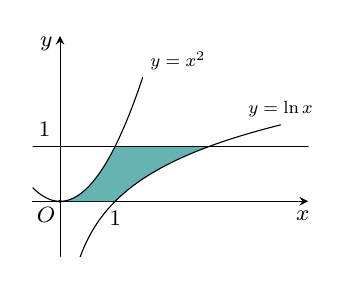
\begin{tikzpicture}[scale=0.7, font=\footnotesize, line join=round,
        line cap=round, >=stealth]
        \pgfmathsetmacro\e{2.718}
        \def \xmin{-0.5}
        \def \xmax{4}
        \def \ymin{-1}
        \def \ymax{3}
        \draw[->] (\xmin,0)--(\xmax+0.5,0) node[shift=(-110:0.2)] {$x$};
        \draw[->] (0,\ymin)--(0,\ymax) node[shift=(-150:0.2)] {$y$};
        \fill (0,0) circle(1pt) node[shift=(-135:0.25)]{$O$};
        \fill [teal, opacity=0.6] (0,0) plot[domain=0:1, samples=100] (\x,{(\x)^2}) -- (\e,1)-- plot[domain=\e:1, samples=100] (\x,{ln ((\x))})-- (1,0) -- cycle;
        \clip (\xmin,\ymin) rectangle (\xmax+1,\ymax);
        \draw[smooth,samples=100,domain=\xmin:1.5] plot(\x,{(\x)^2}) node[above right,scale=0.8] {$y=x^2$};
        \draw[smooth,samples=100,domain=0.25:\xmax] plot(\x,{ln ((\x))}) node[above,scale=0.8] {$y=\ln x$} ;
        \draw (\xmin,1)--(\xmax+0.5,1);
        \node[below] at (1,0) {$1$};
        \node[above left] at (0,1) {$1$};
    \end{tikzpicture}
}
%    \loigiai{Ta có
%        \[S=\displaystyle \int \limits_0^1 x^2 \ \mathrm{d}x + \int \limits_1^\mathrm{e} \ln x \ \mathrm{d}x=\mathrm{e}-\dfrac{5}{3}.\]}
\end{ex}
\begin{ex}%[Pj27--2-TT-THPTQGNH24-25--TeamTeXHoa--Phạm Hoàng Đăng]%[2D4H3-1] 
    \immini[thm]{
        Cho hàm số $f(x)=-x^3+3x^2+2$ có đồ thị $(\mathscr{C})$ như hình vẽ. Tính diện tích $S$ có hình phẳng được tô như trong hình.
        \choice
        {$S=10$}
        {\True $S=\dfrac{39}{4}$}
        {$S=\dfrac{41}{4}$}
        {$S=13$}
    }{
        \begin{tikzpicture}[>=stealth,yscale=0.4,xscale=.7,font=\footnotesize]
            \def\xmin{-1.5};\def\xmax{4.5};\def\ymin{-1};\def\ymax{6.5};
            \draw[->] (\xmin,0)--(\xmax,0) node[below right] {$x$};
            \draw[->] (0,\ymin)--(0,\ymax) node[left] {$y$};
            \begin{scope}
                \clip (\xmin,\ymin) rectangle (\xmax,\ymax);
                \draw[samples=200,domain=\xmin:\xmax,smooth,variable=\x] plot (\x,{-(\x)^3+3*(\x)^2+2});
                \draw[samples=200,domain=\xmin:\xmax,smooth,variable=\x] plot (\x,{2/3*(\x)});
                \fill[pattern=north west lines]
                plot[domain=0:3] (\x, {-(\x)^3+3*(\x)^2+2})--(3,2) --       
                plot[domain=3:0] (\x, {2/3*(\x)})--(0,0) -- cycle;               
            \end{scope}
            \draw[dashed] (3,0)|-(0,2);
            \draw[fill=black] (0,0)circle(1.2pt) node [below right] {$O$}
            (0,2)circle(1.2pt) node [below left] {$2$}
            (3,0)circle(1.2pt) node [below] {$3$}
            ;
        \end{tikzpicture}
    }
%    \loigiai{
%        Đường thẳng đi qua điểm $(0 ; 0)$, $(3 ; 2)$ có phương trình là $y=\dfrac{2}{3} x$.\\
%        Diện tích cần tính là $S=\displaystyle\int\limits_0^3\left(-x^3+3 x^2+2-\dfrac{2}{3} x\right)\mathrm{\,d}x=\left.\left(-\dfrac{x^4}{4}+x^3+2 x-\frac{1}{3} x^2\right)\right|_0 ^3=\dfrac{39}{4}$.
%        
%    }
\end{ex}
 
     \begin{ex}[THPT Trần Phú - Vĩnh Phúc - 2025]
         Một vật chuyển động với vận tốc $v(t) = 4t + 8$ (m/s), với thời gian $t$ tính bằng giây. Tính quãng đường vật đi được trong khoảng thời gian từ $t = 8$ đến $t = 10$.
         \choice
         {$89\text{ (m)}$}
         {$87\text{ (m)}$}
         {$86\text{ (m)}$}
         {\True $88\text{ (m)}$}
          \loigiai{
              Quãng đường vật đi được trong khoảng thời gian từ $t = 8$ đến $t = 10$ là:
              $$S = \int\limits_8^{10} v(t)\mathrm{d}t = \int\limits_8^{10} (4t + 8)\mathrm{d}t = \left(2t^2 + 8t\right)\Big|_8^{10} = (2\cdot 10^2 + 8\cdot 10) - (2\cdot 8^2 + 8\cdot 8) = 280 - 192 = 88 \text{ (m)}.$$
              }
     \end{ex}
\begin{ex}Cho hàm số $f(x)$ thỏa mãn $f'(x) = e^x + \sin x$ và $f(0)=2$. Gọi $F(x)$ là một họ nguyên hàm của $f(x)$. Xét tính đúng sai của các mệnh đề sau:
 \choiceTF
 {\True Hàm số $f(x)$ là một nguyên hàm của hàm số $g(x) = e^x + \sin x$}
 {Phương trình $f(x) - e^x = 0$ có hai nghiệm thuộc khoảng $(0; 2\pi)$}
 {Họ nguyên hàm của hàm số $f(x)$ là $F(x) = e^x + \sin x + 2x + C$}
 {Nếu $F(0) = 0$ thì $F\left(\frac{\pi}{2}\right) + f\left(\frac{\pi}{2}\right) = e^{\frac{\pi}{2}} + \pi$}
 \loigiai{Ta có $f(x) = \int (e^x + \sin x)\mathrm{d}x = e^x - \cos x + C$.Vì $f(0) = 2 \Rightarrow e^0 - \cos 0 + C = 2 \Rightarrow 1 - 1 + C = 2 \Rightarrow C = 2$.Do đó $f(x) = e^x - \cos x + 2$.\begin{itemize}\item \textbf{a) Đúng:} Vì $f'(x) = e^x + \sin x = g(x)$.\item \textbf{b) Sai:} Phương trình $f(x) - e^x = 0 \Leftrightarrow e^x - \cos x + 2 - e^x = 0 \Leftrightarrow \cos x = 2$ (vô nghiệm).\item \textbf{c) Sai:} Ta có $F(x) = \int (e^x - \cos x + 2)\mathrm{d}x = e^x - \sin x + 2x + C$.\item \textbf{d) Sai:} Với $F(0) = 0 \Rightarrow e^0 - \sin 0 + 0 + C_1 = 0 \Rightarrow C_1 = -1$.Khi đó $F(x) = e^x - \sin x + 2x - 1$.Ta có $F\left(\frac{\pi}{2}\right) = e^{\frac{\pi}{2}} - \sin\frac{\pi}{2} + 2\cdot\frac{\pi}{2} - 1 = e^{\frac{\pi}{2}} + \pi - 2$.Mặt khác $f\left(\frac{\pi}{2}\right) = e^{\frac{\pi}{2}} - \cos\frac{\pi}{2} + 2 = e^{\frac{\pi}{2}} + 2$.Suy ra $F\left(\frac{\pi}{2}\right) + f\left(\frac{\pi}{2}\right) = 2e^{\frac{\pi}{2}} + \pi \neq e^{\frac{\pi}{2}} + \pi$.\end{itemize}}
 \dotlineEX{3}
 \end{ex}
\begin{ex}Cho hàm số $f(x)$ là một nguyên hàm của $g(x) = x^2 - 4x + a$. Biết $f'(2) = -9$. Xét tính đúng sai của các mệnh đề sau:
 \choiceTF
 {$a = -3$}
 {Tiếp tuyến của đồ thị hàm số $y = f(x)$ tại điểm $x_0 = -1$ có hệ số góc bằng $-1$}
 {Hàm số $f(x)$ đồng biến trên khoảng $(-1; 5)$}
 {\True Nếu $f(3) = 5$ thì $f(6) = -1$}
 \loigiai{Vì $f(x)$ là nguyên hàm của $g(x)$ nên $f'(x) = g(x) = x^2 - 4x + a$.Ta có $f'(2) = -9 \Leftrightarrow 2^2 - 4\cdot 2 + a = -9 \Leftrightarrow a = -5$.Suy ra $f'(x) = x^2 - 4x - 5$.\begin{itemize}\item \textbf{a) Sai:} Vì $a = -5$.\item \textbf{b) Sai:} Hệ số góc tiếp tuyến tại $x_0 = -1$ là $k = f'(-1) = (-1)^2 - 4(-1) - 5 = 0$.\item \textbf{c) Sai:} Ta có $f'(x) = 0 \Leftrightarrow \left[ \begin{array}{l} x = -1 \\ x = 5 \end{array} \right.$.Xét dấu $f'(x)$ ta thấy $f'(x) < 0$ với mọi $x \in (-1; 5)$. Do đó hàm số nghịch biến trên $(-1; 5)$.\item \textbf{d) Đúng:} Ta có $f(x) = \int (x^2 - 4x - 5)\mathrm{d}x = \frac{x^3}{3} - 2x^2 - 5x + C$.Với $f(3) = 5 \Leftrightarrow \frac{3^3}{3} - 2\cdot 3^2 - 5\cdot 3 + C = 5 \Leftrightarrow -24 + C = 5 \Leftrightarrow C = 29$.Khi đó $f(x) = \frac{x^3}{3} - 2x^2 - 5x + 29 \Rightarrow f(6) = \frac{6^3}{3} - 2\cdot 6^2 - 5\cdot 6 + 29 = -1$.\end{itemize}}
 \dotlineEX{4}
 \end{ex}
\begin{ex}
 Cho hàm số $f(x)$ liên tục, thoả mãn $f(x) = 2x - xf'(x)$ với mọi $x \neq 0$.
 \choiceTF
 {\True $[xf(x)]' = 2x$}
 {\True Công thức của hàm số $f(x)$ là $f(x) = \frac{x^2+C}{x}$}
 {Nếu $f(2) = -1$ thì $C = -5$}
 {\True Một nguyên hàm của $x^2f(x)$ trên $\mathbb{R} \setminus \{0\}$ là $\frac{x^4}{4} + \frac{Cx^2}{2} + 1$}
 \loigiai{
 a) Ta có $f(x) = 2x - xf'(x) \Leftrightarrow f(x) + xf'(x) = 2x \Leftrightarrow [xf(x)]' = 2x$. Vậy a đúng.\\
 b) Lấy nguyên hàm hai vế ta được: $\int [xf(x)]' \mathrm{d}x = \int 2x \mathrm{d}x \Rightarrow xf(x) = x^2 + C \Rightarrow f(x) = \frac{x^2+C}{x}$. Vậy b đúng.\\
 c) Thay $x = 2$ vào hàm số, ta có $f(2) = \frac{2^2+C}{2} = -1 \Rightarrow 4+C = -2 \Rightarrow C = -6$. Vậy c sai.\\
 d) Ta có $x^2 f(x) = x^2 \cdot \frac{x^2+C}{x} = x^3 + Cx$. \\
 Họ nguyên hàm của hàm số này là: $\int (x^3 + Cx) \mathrm{d}x = \frac{x^4}{4} + \frac{Cx^2}{2} + C_1$. \\
 Bằng cách chọn hằng số $C_1 = 1$, ta được một nguyên hàm là $\frac{x^4}{4} + \frac{Cx^2}{2} + 1$. Vậy d đúng.
 }
\end{ex}
 \dotlineEX{3}
\begin{ex}%[389394]%[MĐ2]
 Một viên đạn được bắn thẳng đứng lên trên từ mặt đất. Vận tốc tại giây thứ $t$ là $v(t) = 166,6 - 9,8t$ ($\text{m}/\text{s}$). Xét tính đúng sai của các mệnh đề sau:
 \choiceTF
 {\True Sau $t=5$ giây độ cao của viên đạn là $710,5$ mét}
 {Sau $10$ s vận tốc của viên đạn là $66,8$ m/s}
 {\True Tại thời điểm $t=17$ (s) thì viên đạn đạt độ cao lớn nhất}
 {Độ cao lớn nhất mà viên đạn đạt được là $1411,2$ mét}
 \loigiai{
 Hàm độ cao $h(t) = \displaystyle\int v(t)\,\text{d}t = 166,6t - 4,9t^2$ (do $h(0)=0$).\\
 a) $h(5) = 166,6(5) - 4,9(5^2) = 710,5$ m. (Đúng)\\
 b) $v(10) = 166,6 - 9,8(10) = 68,6$ m/s. (Sai)\\
 c) Độ cao cực đại khi $v(t)=0 \Rightarrow 166,6 - 9,8t = 0 \Rightarrow t = 17$ s. (Đúng)\\
 d) $h_{max} = h(17) = 166,6(17) - 4,9(17^2) = 1416,1$ m. (Sai)
 }
  \dotlineEX{3}
\end{ex}
\begin{ex}%[389395]%[MĐ2]%[SGK Cánh Diều]
 Tại một lễ hội dân gian, sự thay đổi lượng khách tham dự được biểu diễn bằng hàm số $B'(t)=20t^3 - 300t^2 + 1000t$, trong đó $t$ tính bằng giờ ($0 \le t \le 15$), $B'(t)$ tính bằng khách/giờ. Sau một giờ, $500$ người đã có mặt tại lễ hội. Xét tính đúng sai của các mệnh đề sau:
 \choiceTF
 {Công thức của hàm số $B(t)$ biểu diễn số lượng khách tham dự lễ hội là: $B(t)=5t^4 - 100t^3 + 500t^2$ với $0 \le t \le 15$}
 {\True Sau $3$ giờ sẽ có $2300$ khách tham dự lễ hội}
 {Số lượng khách tham dự lễ hội lớn nhất là $3200$ người}
 {Tại thời điểm $t=6$ (h) thì tốc độ thay đổi lượng khách tham dự lễ hội là lớn nhất}
 \loigiai{
 Ta có $B(t) = \displaystyle\int B'(t) \text{d}t = 5t^4 - 100t^3 + 500t^2 + C$.\\
 Vì $B(1) = 500 \Rightarrow 5 - 100 + 500 + C = 500 \Rightarrow C = 95$.\\
 Vậy $B(t) = 5t^4 - 100t^3 + 500t^2 + 95$.\\
 a) Sai vì thiếu hằng số $C=95$.\\
 b) $B(3) = 5 \cdot 3^4 - 100 \cdot 3^3 + 500 \cdot 3^2 + 95 = 2300$. (Đúng)\\
 c) Xét $B'(t)=0 \Leftrightarrow 20t(t-5)(t-10)=0 \Rightarrow t=5, t=10$. Lập bảng biến thiên trên $[0;15]$, ta thấy $B(t)$ đạt GTLN tại $t=15$, $B(15) = 28220$. (Sai)\\
 d) Tốc độ thay đổi là $B'(t)$. Xét $B''(t) = 60t^2 - 600t + 1000 = 0 \Rightarrow t \approx 2,1$ hoặc $t \approx 7,9$. Tại $t=6$ không phải điểm cực trị của $B'(t)$. (Sai)
 }
  \dotlineEX{1}
\end{ex}
\begin{ex}%[389397]%[MĐ2]%[SGK Cánh Diều]
 Cây cà chua khi trồng có chiều cao $5$ cm. Sự thay đổi chiều cao sau khi trồng được cho bởi hàm số $h'(t)=-0,1t^3 + t^2$, trong đó $t$ tính theo tuần ($0 \le t \le 12$), $h'(t)$ tính bằng cm/tuần. Gọi $h(t)$ là độ cao của cây ở tuần thứ $t$. Xét tính đúng sai của các mệnh đề sau:
 \choiceTF
 {\True Công thức xác định hàm số $h(t)$ là $h(t)=-0,025t^4 + \dfrac{1}{3}t^3 + 5$ ($0 \le t \le 11$)}
 {Sau $4$ năm cây cà chua sẽ cao $44,6$ cm}
 {Chiều cao tối đa của cây cà chua đó là $62,6$ cm}
 {\True Vào thời điểm cây cà chua đó phát triển nhanh nhất thì cây cà chua sẽ cao khoảng $54,4$ cm}
 \loigiai{
 a) $h(t) = \displaystyle\int (-0,1t^3 + t^2) \text{d}t = -0,025t^4 + \dfrac{1}{3}t^3 + C$. Vì $h(0)=5 \Rightarrow C=5$. (Đúng)\\
 b) Đề bài cho $t$ tính theo tuần, mệnh đề ghi "năm" là sai đơn vị. Hơn nữa $h(4) \approx 19,9$ cm. (Sai)\\
 c) $h'(t)=0 \Rightarrow t=10$. GTLN của $h(t)$ trên $[0;12]$ đạt tại $t=10$, $h(10) = -250 + \dfrac{1000}{3} + 5 \approx 88,3$ cm. (Sai)\\
 d) Cây phát triển nhanh nhất khi $h'(t)$ max. $h''(t) = -0,3t^2 + 2t = 0 \Rightarrow t = \dfrac{20}{3}$ tuần. Khi đó $h\left(\dfrac{20}{3}\right) = -0,025\left(\dfrac{20}{3}\right)^4 + \dfrac{1}{3}\left(\dfrac{20}{3}\right)^3 + 5 \approx 54,4$ cm. (Đúng)
 }
  \dotlineEX{1}
\end{ex}
\begin{ex}[Trần Phú Lần 2 - Hà Nội-2026]%[Câu 3]
 Một miếng thịt sống được lấy ra khỏi ngăn đá của tủ lạnh và để trên bàn để rã đông. Nhiệt độ của miếng thịt khi nó được lấy ra khỏi ngăn đá là $-4^\circ\text{C}$ và sau $t$ giờ nhiệt độ của miếng thịt tăng với tốc độ $T'(t) = 7e^{-0,35t}$ ($^\circ\text{C}/\text{giờ}$). Miếng thịt này được rã đông khi nhiệt độ của nó đạt đến $10^\circ\text{C}$.
 \choiceTF
 {Tại thời điểm $2$h tính từ lúc lấy thịt ra khỏi ngăn đá, tốc độ thay đổi nhiệt độ của miếng thịt khoảng $3,48^\circ\text{C}/\text{giờ}$ (làm tròn kết quả đến hàng phần trăm)}
 {\True Nhiệt độ miếng thịt tính từ thời điểm được lấy khỏi ngăn đá là $T(t) = 7e^{-0,35t} - 11$ ($^\circ\text{C}$)}
 {Tính từ lúc lấy thịt ra khỏi ngăn đá, cần $3,44$ giờ để miếng thịt được rã đông (làm tròn kết quả đến hàng phần trăm của giờ)}
 {Tính từ lúc lấy thịt ra khỏi ngăn đá, nhiệt độ của miếng thịt vào khoảng $0^\circ\text{C}$ sau $36$ phút (làm tròn kết quả đến hàng đơn vị của phút)}
 \loigiai{
 \begin{itemize}
 \item[\textbf{a)}] $T'(2) = 7e^{-0,35 \cdot 2} \approx 3,4758 \approx 3,48 \Rightarrow$ \textbf{Đúng}.
 \item[\textbf{b)}] $T(t) = \displaystyle\int 7e^{-0,35t} \text{d}t = -20e^{-0,35t} + C$. \\
 Vì $T(0) = -4 \Rightarrow -20 + C = -4 \Rightarrow C = 16$. \\
 Vậy $T(t) = -20e^{-0,35t} + 16 \Rightarrow$ \textbf{Sai}.
 \item[\textbf{c)}] Giải $T(t) = 10 \Leftrightarrow -20e^{-0,35t} + 16 = 10 \Leftrightarrow e^{-0,35t} = 0,3$. \\
 $\Rightarrow t = \frac{\ln(0,3)}{-0,35} \approx 3,4399 \approx 3,44 \Rightarrow$ \textbf{Đúng}.
 \item[\textbf{d)}] $36 \text{ phút} = 0,6 \text{ giờ}$. $T(0,6) = -20e^{-0,35 \cdot 0,6} + 16 \approx -0,21 \approx 0 \Rightarrow$ \textbf{Đúng}.
 \end{itemize}
 }
  \dotlineEX{3}
\end{ex}
\begin{ex}%[389396]%[MĐ2]%[SGK Cánh Diều]
 Một ô tô đang chạy với tốc độ $72$ km/h thì người lái xe bất ngờ phát hiện chướng ngại vật cách đó $80$ m. Người lái xe phản ứng một giây sau đó bằng cách đạp phanh khẩn cấp. Kể từ thời điểm này, ô tô chuyển động chậm dần đều với tốc độ $v(t)=-10t + 30$ (m/s), trong đó $t$ là thời gian tính bằng giây kể từ lúc đạp phanh. Gọi $s(t)$ là quãng đường xe ô tô đi được trong $t$ (giây) kể từ lúc đạp phanh. Xét tính đúng sai của các mệnh đề sau:
 \choiceTF
 {Thời gian kể từ lúc đạp phanh đến khi xe ô tô dừng hẳn là $15$ s}
 {\True Công thức biểu diễn hàm số $s(t)$ là: $s(t)=-5t^2 + 30t$ ($0 \le t \le 3$)}
 {Quãng đường xe ô tô đã di chuyển kể từ lúc người lái xe phát hiện chướng ngại vật trên đường đến khi xe ô tô dừng hẳn là $45$ mét}
 {\True Xe ô tô sẽ không gặp tai nạn do va chạm với chướng ngại vật trên đường}
 \loigiai{
 Đổi $72$ km/h = $20$ m/s.\\
 a) Xe dừng hẳn khi $v(t)=0 \Rightarrow -10t + 30 = 0 \Rightarrow t=3$ s. (Sai)\\
 b) $s(t) = \displaystyle\int (-10t + 30) \text{d}t = -5t^2 + 30t + C$. Với $s(0)=0 \Rightarrow C=0$. Vậy $s(t) = -5t^2 + 30t$. (Đúng)\\
 c) Quãng đường phản ứng (1s): $s_1 = 20 \cdot 1 = 20$ m. Quãng đường phanh: $s(3) = -5 \cdot 3^2 + 30 \cdot 3 = 45$ m. Tổng quãng đường: $20 + 45 = 65$ m. (Sai)\\
 d) Tổng quãng đường $65$ m $< 80$ m nên không đâm vào chướng ngại vật. (Đúng)
 }
\end{ex}
\begin{ex}[KSCL12-Sở Hà Nội-2026]
 Một người đang điều khiển ô tô chạy trên đường cao tốc. Khi cách trạm thu phí $1000$ m, tốc độ của ô tô là $90$ km/h. Sau đó $20$ giây, người điều khiển ô tô bắt đầu giảm tốc với tốc độ $v(t) = at + b$ (m/s), trong đó $t$ là thời gian tính bằng giây kể từ khi bắt đầu giảm tốc và $v(t) > 0$ với mọi $t \in [0;30]$. Sau $30$ giây kể từ khi bắt đầu giảm tốc, ô tô đến trạm thu phí.
 \choiceTF
 {\True Quãng đường từ vị trí ô tô bắt đầu giảm tốc đến trạm thu phí là $500$ m}
 {Giá trị của $b$ là $90$}
 {\True Giá trị của $a$ là $-\dfrac{5}{9}$}
 {\True Tốc độ tối đa cho phép của phương tiện khi qua trạm thu phí là $30$ km/h. Người điều khiển ô tô đó đã tuân thủ đúng tốc độ quy định khi qua trạm thu phí}
 \loigiai{
 Đổi $90$ km/h $= 25$ m/s.
 \begin{itemize}
 \item Trong $20$ giây đầu (trước khi giảm tốc), ô tô đi được quãng đường là: $s_1 = 25 \cdot 20 = 500$ (m).
 \item Quãng đường từ vị trí bắt đầu giảm tốc đến trạm thu phí là: $s_2 = 1000 - 500 = 500$ (m). Vậy \textbf{a) Đúng}.
 \item Tại thời điểm bắt đầu giảm tốc ($t=0$), vận tốc là $v(0) = 25$ m/s. Suy ra $a(0) + b = 25 \Rightarrow b = 25$. Vậy \textbf{b) Sai}.
 \item Quãng đường đi được trong $30$ giây giảm tốc là:
 $$s_2 = \int_{0}^{30} (at + 25) \, \mathrm{d}t = \left. \left( \dfrac{at^2}{2} + 25t \right) \right|_0^{30} = 450a + 750.$$
 Theo bài ra $s_2 = 500$, nên $450a + 750 = 500 \Leftrightarrow 450a = -250 \Leftrightarrow a = -\dfrac{5}{9}$. Vậy \textbf{c) Đúng}.
 \item Vận tốc của ô tô khi đến trạm thu phí ($t=30$):
 $v(30) = -\dfrac{5}{9} \cdot 30 + 25 = -\dfrac{50}{3} + 25 = \dfrac{25}{3}$ (m/s).
 Đổi sang km/h: $\dfrac{25}{3} \cdot 3,6 = 30$ (km/h).
 Vì vận tốc bằng đúng tốc độ tối đa cho phép ($30$ km/h) nên người lái xe đã tuân thủ đúng quy định. Vậy \textbf{d) Đúng}.
 \end{itemize}
 }
  \dotlineEX{2}
\end{ex}
\begin{ex}[Sở Lạng Sơn - 2026]%[2D3Y1-1]
 Giả sử rằng khi được $t$ năm tuổi, một máy công nghiệp $A$ tạo ra doanh thu với tốc độ $R'(t)=588-3t^2$ (triệu đồng/năm), thời điểm $t=0$ tính từ lúc máy $A$ bắt đầu hoạt động. Biết rằng chi phí biên cho vận hành và bảo trì là $C'(t)=48+12t^2$ (triệu đồng/năm), ở đây $C(t)$ là chi phí vận hành và bảo trì của máy $A$ khi nó được $t$ năm tuổi. Khi đó:
 \choiceTF
 {\True Doanh thu sau $10$ năm của máy $A$ là $\displaystyle\int_0^{10} (588-3t^2) \text{d}t$ (triệu đồng)}
 {\True Tổng chi phí vận hành và bảo trì của máy $A$ trong $6$ năm là $1152$ (triệu đồng)}
 {Tuổi thọ hữu ích của một máy là số năm $T$ trước khi lợi nhuận (bằng doanh thu trừ chi phí) mà nó tạo ra bắt đầu giảm. Tuổi thọ hữu ích của máy $A$ này là $8$ năm}
 {Lợi nhuận do máy $A$ tạo ra trong suốt thời gian tuổi thọ hữu ích của nó là $2180$ (triệu đồng)}
 \loigiai{
 a) Doanh thu sau $10$ năm được tính bởi tích phân của tốc độ doanh thu từ $0$ đến $10$: $R(10) = \displaystyle\int_0^{10} R'(t) \text{d}t = \int_0^{10} (588-3t^2) \text{d}t$. Vậy khẳng định này \textbf{Đúng}.\\
 b) Tổng chi phí trong $6$ năm: $C(6) = \displaystyle\int_0^6 (48+12t^2) \text{d}t = \left. (48t + 4t^3) \right|_0^6 = 48(6) + 4(6^3) = 288 + 864 = 1152$. Vậy khẳng định này \textbf{Đúng}.\\
 c) Gọi $P(t)$ là lợi nhuận: $P(t) = R(t) - C(t) \Rightarrow P'(t) = R'(t) - C'(t)$.\\
 Lợi nhuận bắt đầu giảm khi $P'(t) < 0 \Leftrightarrow R'(t) < C'(t)$.\\
 Xét phương trình $R'(t) = C'(t) \Leftrightarrow 588 - 3t^2 = 48 + 12t^2 \Leftrightarrow 15t^2 = 540 \Leftrightarrow t^2 = 36 \Rightarrow t = 6$ (vì $t > 0$).\\
 Vậy tuổi thọ hữu ích là $T = 6$ năm. Khẳng định này \textbf{Sai}.\\
 d) Lợi nhuận trong suốt tuổi thọ hữu ích ($T=6$):\\
 $P(6) = \displaystyle\int_0^6 [R'(t) - C'(t)] \text{d}t = \int_0^6 (540 - 15t^2) \text{d}t = \left. (540t - 5t^3) \right|_0^6 = 540(6) - 5(6^3) = 3240 - 1080 = 2160$.\\
 Vậy khẳng định này \textbf{Sai}.
 }
\end{ex}
\begin{ex}
 Giả sử chi phí mua và bảo trì một thiết bị trong $x$ năm có thể được mô hình hóa theo công thức $C = 5000 \left( 25 + 3 \int_0^x t^{\frac{1}{4}} \mathrm{d}t \right)$. Các mệnh đề sau đúng hay sai?
 \choiceTF
 {Chi phí mua $1$ sản phẩm là $100.000$ đồng}
 {Chi phí bảo trì năm đầu tiên của $1$ sản phẩm là $12.000$ đồng}
 {Sau $6,5$ năm thì số tiền mua một sản phẩm bằng số tiền bảo trì sản phẩm đó}
 {Nếu một nhà đầu tư có $10$ triệu, thì họ có thể mua và bảo trì tối đa $30$ sản phẩm trong $10$ năm}
 \loigiai{
 Công thức tổng quát: $C = 5000 \left( 25 + 3 \cdot \frac{4}{5}x^{\frac{5}{4}} \right) = 125.000 + 12.000 x^{\frac{5}{4}}$.
 \begin{itemize}
 \item Chi phí mua ban đầu ứng với $x=0$: $C(0) = 125.000$ đồng. Vậy \textbf{a) Sai}.
 \item Chi phí bảo trì năm đầu tiên ($x=1$): $12.000 \cdot (1)^{\frac{5}{4}} = 12.000$ đồng. Vậy \textbf{b) Đúng}.
 \item Tiền mua bằng tiền bảo trì khi: $125.000 = 12.000 x^{\frac{5}{4}} \Leftrightarrow x^{\frac{5}{4}} = \frac{125}{12} \approx 10,4 \Rightarrow x \approx (10,4)^{0,8} \approx 6,48$ (năm). Làm tròn là $6,5$ năm. Vậy \textbf{c) Đúng}.
 \item Chi phí $1$ sản phẩm trong $10$ năm: $C(10) = 125.000 + 12.000 \cdot 10^{\frac{5}{4}} \approx 125.000 + 12.000 \cdot 17,78 \approx 338.360$ đồng.
 Với $10.000.000$ đồng, số sản phẩm tối đa là: $\frac{10.000.000}{338.360} \approx 29,55$. 
 Vậy chỉ mua được tối đa $29$ sản phẩm. \textbf{d) Sai}.
 \end{itemize}
 }
\end{ex}
\begin{ex}
 Một quần thể vi khuẩn $(A)$ có số lượng cá thể là $P(t)$, trong đó $t$ là thời gian tính bằng phút kể từ khi bắt đầu quan sát. Nghiên cứu cho thấy số lượng vi khuẩn $(A)$ thay đổi với tốc độ là $P'(t) = 300\mathrm{e}^{0,1t} + 200\mathrm{e}^{-0,04t}$. Lúc bắt đầu quan sát, quần thể $(A)$ có $300\,000$ vi khuẩn. Sau $15$ phút, một quần thể vi khuẩn $(B)$ xuất hiện và có tốc độ tăng trưởng là $Q'(u) = 500\mathrm{e}^{0,2u}$, với $u$ là thời gian tính bằng phút kể từ khi vi khuẩn $(B)$ xuất hiện. Sau khi vi khuẩn $(B)$ xuất hiện $9$ phút thì số lượng vi khuẩn hai quần thể bằng nhau.
 \choiceTF
 { $P'(0) = 0$}
 {\True $P(0) = 300\,000$}
 {\True Sau $24$ phút kể từ khi bắt đầu quan sát, số lượng vi khuẩn $(A)$ là $333\,155$ con}
 {Số lượng vi khuẩn $(B)$ ở thời điểm bắt đầu xuất hiện không vượt quá $320\,000$ con}
 \loigiai{
 \begin{itemize}
 \item Số lượng cá thể quần thể $(A)$ là:
 $$P(t) = \int P'(t)\mathrm{d}t = \int \left(300\mathrm{e}^{0,1t} + 200\mathrm{e}^{-0,04t}\right)\mathrm{d}t = 3000\mathrm{e}^{0,1t} - 5000\mathrm{e}^{-0,04t} + C_1$$
 Ban đầu quần thể $(A)$ có $300\,000$ vi khuẩn nên:
 $$P(0) = 300\,000 \Leftrightarrow 3000 - 5000 + C_1 = 300\,000 \Rightarrow C_1 = 302\,000$$
 Vậy $P(t) = 3000\mathrm{e}^{0,1t} - 5000\mathrm{e}^{-0,04t} + 302\,000$.
 \item Xét ý a: $P'(0) = 300\mathrm{e}^0 + 200\mathrm{e}^0 = 500 \neq 0$. (Sai)
 \item Xét ý b: Theo giả thiết ban đầu $P(0) = 300\,000$. (Đúng)
 \item Xét ý c: Sau $24$ phút, số lượng vi khuẩn $(A)$ là:
 $$P(24) = 3000\mathrm{e}^{2,4} - 5000\mathrm{e}^{-0,96} + 302\,000 \approx 333\,155 \text{ (con)}.$$
 (Đúng)
 \item Xét ý d: Số lượng cá thể quần thể $(B)$ là:
 $$Q(u) = \int Q'(u)\mathrm{d}u = \int 500\mathrm{e}^{0,2u}\mathrm{d}u = 2500\mathrm{e}^{0,2u} + C_2$$
 Vi khuẩn $(B)$ xuất hiện $9$ phút ứng với thời gian quan sát là $t = 15 + 9 = 24$ phút. Khi đó hai quần thể bằng nhau:
 $$Q(9) = P(24) \Leftrightarrow 2500\mathrm{e}^{1,8} + C_2 \approx 333\,155,07 \Rightarrow C_2 \approx 318\,030,95$$
 Số lượng vi khuẩn $(B)$ lúc bắt đầu xuất hiện ($u=0$) là:
 $$Q(0) = 2500\mathrm{e}^0 + C_2 = 2500 + 318\,030,95 \approx 320\,531 \text{ (con)}.$$
 Ta thấy $320\,531 > 320\,000$ nên số lượng vi khuẩn $(B)$ ban đầu đã vượt quá $320\,000$ con. (Sai)
 \end{itemize}
 }
\end{ex}
\begin{ex}
 Một con sư tử đang đuổi theo một con ngựa vằn và chúng cùng chạy trên một đường thẳng. Ngựa vằn đã nhận ra sư tử khi sư tử cách nó khoảng $40 \text{ m}$. Từ thời điểm này, sư tử đuổi theo ngựa vằn với tốc độ $v_1(t) = 15e^{-0,1t} \text{ (m/s)}$ và ngựa vằn vẫn bỏ chạy với tốc độ $v_2(t) = 20 - 20e^{-0,1t} \text{ (m/s)}$ ($t$ được tính bằng giây với $0 \le t \le 60$).
 \choiceTF
 {Tại thời điểm ban đầu $t=0$ giây, vận tốc của con ngựa vằn là $20 \text{ m/s}$}
 {\True Tốc độ của sư tử giảm dần theo thời gian, trong khi tốc độ của ngựa vằn tăng dần theo thời gian}
 {Sư tử ở gần ngựa vằn nhất khi $v_1'(t) = v_2'(t)$ và khoảng cách ngắn nhất giữa chúng là $1,72 \text{ mét}$ (làm tròn đến hàng phần trăm theo đơn vị mét)}
 {\True Sư tử sẽ không bắt được ngựa vằn và khoảng cách ngắn nhất giữa chúng là $1,92 \text{ mét}$ (làm tròn đến hàng phần trăm theo đơn vị mét)}
 \loigiai{
 a) Tại thời điểm $t=0$, vận tốc của ngựa vằn là $v_2(0) = 20 - 20e^0 = 0 \text{ (m/s)}$. Vậy a sai.\\
 b) Ta xét đạo hàm của các hàm vận tốc: \\
 $v_1'(t) = -1,5e^{-0,1t} < 0, \forall t \ge 0 \Rightarrow$ tốc độ sư tử giảm dần. \\
 $v_2'(t) = 2e^{-0,1t} > 0, \forall t \ge 0 \Rightarrow$ tốc độ ngựa vằn tăng dần. Vậy b đúng.\\
 c) Sư tử ở gần ngựa vằn nhất khi khoảng cách giữa chúng đạt giá trị nhỏ nhất. Khảo sát hàm khoảng cách sẽ cho thấy khoảng cách nhỏ nhất đạt được khi $v_1(t) = v_2(t)$ (hai vận tốc bằng nhau), chứ không phải khi gia tốc bằng nhau ($v_1'(t) = v_2'(t)$). Vậy c sai.\\
 d) Chọn gốc tọa độ tại vị trí ban đầu của sư tử, chiều dương là chiều chuyển động. \\
 Phương trình chuyển động của sư tử: 
 $$x_1(t) = \int_0^t 15e^{-0,1\tau} \mathrm{d}\tau = -150e^{-0,1\tau} \big|_0^t = 150(1 - e^{-0,1t})$$
 Phương trình chuyển động của ngựa vằn: 
 $$x_2(t) = 40 + \int_0^t (20 - 20e^{-0,1\tau}) \mathrm{d}\tau = 40 + (20\tau + 200e^{-0,1\tau}) \big|_0^t = 20t + 200e^{-0,1t} - 160$$
 Khoảng cách giữa hai con vật tại thời điểm $t$ là: 
 $$d(t) = x_2(t) - x_1(t) = 20t + 200e^{-0,1t} - 160 - 150 + 150e^{-0,1t} = 20t + 350e^{-0,1t} - 310$$
 Khoảng cách này đạt nhỏ nhất khi $d'(t) = 0 \Leftrightarrow v_2(t) - v_1(t) = 0 \Leftrightarrow 20 - 35e^{-0,1t} = 0 \Leftrightarrow e^{-0,1t} = \frac{4}{7}$. \\
 $\Rightarrow -0,1t = \ln\frac{4}{7} \Rightarrow t = 10\ln\frac{7}{4}$. \\
 Thế $t$ vào hàm khoảng cách, ta có khoảng cách ngắn nhất là: 
 $$d_{min} = 20\left(10\ln\frac{7}{4}\right) + 350 \cdot \frac{4}{7} - 310 = 200\ln\frac{7}{4} - 110 \approx 1,92 \text{ (m)}$$
 Vì khoảng cách ngắn nhất là $1,92 \text{ m} > 0$ nên sư tử sẽ không bắt được ngựa vằn. Vậy d đúng.
 }
\end{ex}
\begin{ex}
 \immini[thm]{Thành phố $X$ theo dõi tốc độ gia tăng dân số của hai khu vực $A$ và $B$ trong thời gian $6$ năm. Hình vẽ sau mô tả tốc độ gia tăng dân số của hai khu vực trên trong $6$ năm, với đơn vị trên trục $Ot$ tính bằng năm, $t = 0$ ứng với mốc từ đầu năm $2019$. Đơn vị trên trục $Oy$ biểu diễn ngàn người tăng thêm mỗi năm.\\
 Khu vực $A$ có tốc độ gia tăng dân số theo thời gian được mô tả bởi hàm
 $P_A'(t) = -\frac{1}{2}t^2 + 2t + 8.$\\
 Khu vực $B$ có tốc độ gia tăng dân số theo thời gian được mô tả bởi hàm $P_B'(t) = a - \frac{1}{2}t$.\\
 Biết rằng $P_A(t)$, $P_B(t)$ lần lượt biểu diễn tổng số dân tăng thêm tại khu vực $A$ và $B$ sau $t$ năm.
 }{
\begin{tikzpicture}[line join = round, line cap = round, >=stealth,
    declare function={
        f(\x)=-0.5*(\x)^2+2*\x+8;
        g(\x)=-0.5*\x+8;
    },x=.7cm,y=.5cm]
    \draw[->] (-1,0)--(7,0)node[below]{$t$};
    \draw[->] (0,-1)--(0,11)node[left]{$y$};
    \draw (0,0) node[below left]{$O$};
    \fill[pattern = north east lines] (0,8) plot[smooth,domain=0:5](\x,{f(\x)})--cycle;
    \draw (0,8) --(6,{g(6)})node[right]{$P'_B(t)$};
    \draw(0,8) plot[smooth,domain=0:6](\x,{f(\x)})node[ right]{$P'_A(t)$};
    \draw[dashed] (5,0)node[below]{$5$}|-(0,{f(5)});
    \draw[dashed] (6,0)node[below]{$6$}|-(0,{f(6)});
    \draw[dashed] (6,0)|-(0,{g(6)});
    \fill (6,{f(6)}) circle (1pt)
    (6,{g(6)}) circle (1.5pt)
    (5,{f(5)}) circle (1.5pt)
    (0,{f(6)}) circle (1.5pt)
    (0,{g(6)}) circle (1.5pt)
    (0,{f(5)}) circle (1.5pt)
    (0,8)circle (1.5pt) node[left]{$8$};
\end{tikzpicture}
 }
 \choiceTF
 {\True Tốc độ gia tăng dân số của khu vực $A$ với $t = 4$ là $8000$}
 {\True Ta có $P_B'(0) = 8$ và $a = 8$}
 { Dân số của khu vực $A$ tăng thêm từ $0$ đến $5$ năm là $33\,000$}
 { Phần diện tích tô đậm trong hình vẽ biểu diễn sự chênh lệch dân số tăng thêm giữa hai khu vực trong giai đoạn từ $0$ đến $5$ năm là $9\,000$ người}
 \loigiai{
 \begin{itemize}
 \item Xét ý a: Tốc độ gia tăng dân số của khu vực $A$ tại thời điểm $t=4$ là:
 $$P_A'(4) = -\frac{1}{2}\cdot 4^2 + 2\cdot 4 + 8 = 8 \text{ (ngàn người)} = 8000 \text{ (người)}.$$
 Vậy mệnh đề a đúng.
 \item Xét ý b: Quan sát đồ thị, ta thấy đường cong $P_A'(t)$ cắt trục tung tại điểm có tung độ là $P_A'(0) = -\frac{1}{2}\cdot 0^2 + 2\cdot 0 + 8 = 8$. 
 Đường thẳng $P_B'(t)$ cũng đi qua giao điểm này, do đó $P_B'(0) = 8$.
 Thay $t=0$ vào hàm số của khu vực $B$, ta được: $a - \frac{1}{2}\cdot 0 = 8 \Rightarrow a = 8$.
 Vậy mệnh đề b đúng.
 \item Xét ý c: Số dân của khu vực $A$ tăng thêm từ năm $0$ đến năm $5$ là:
 $$\int_0^5 P_A'(t)\mathrm{d}t = \int_0^5 \left(-\frac{1}{2}t^2 + 2t + 8\right)\mathrm{d}t = \left. \left(-\frac{t^3}{6} + t^2 + 8t\right) \right|_0^5 = \frac{265}{6} \approx 44,167 \text{ (ngàn người)}.$$
 Vì $44,167 \text{ ngàn người} \neq 33\,000 \text{ người}$, nên mệnh đề c sai.
 \item Xét ý d: Phương trình hoành độ giao điểm của $P_A'(t)$ và $P_B'(t)$:
 $$-\frac{1}{2}t^2 + 2t + 8 = 8 - \frac{1}{2}t \Leftrightarrow -\frac{1}{2}t^2 + \frac{5}{2}t = 0 \Leftrightarrow \hoac{&t=0\\&t=5.}$$
 Phần diện tích tô đậm biểu diễn sự chênh lệch dân số tăng thêm giữa hai khu vực trong giai đoạn từ $0$ đến $5$ năm là:
 $$S = \int_0^5 \left| P_A'(t) - P_B'(t) \right|\mathrm{d}t = \int_0^5 \left( -\frac{1}{2}t^2 + \frac{5}{2}t \right)\mathrm{d}t = \left. \left( -\frac{t^3}{6} + \frac{5t^2}{4} \right) \right|_0^5 = \frac{125}{12} \approx 10,417 \text{ (ngàn người)}.$$
 Vì $10,417 \text{ ngàn người} \neq 9\,000 \text{ người}$, nên mệnh đề d sai.
 \end{itemize}
 }
  \dotlineEX{4}
\end{ex}
\begin{ex}
 Trong lĩnh vực quản lý tài sản doanh nghiệp, việc đánh giá sự mất giá (khấu hao) của các thiết bị công nghệ cao theo thời gian là rất cần thiết để tối ưu hóa chi phí. Giả sử giá trị của một hệ thống máy chủ trung tâm $y(t)$ (đơn vị: tỉ đồng) sau $t$ tháng ($t \ge 0$) kể từ lúc mua thỏa mãn $y(t) > 0$ và $y'(t) = k \cdot y(t)$ ($t \ge 0$), trong đó $k$ là hằng số khác không. Theo dõi định giá tài sản, sau $5$ tháng sử dụng, giá trị hệ thống máy chủ là $3$ tỉ đồng. Sau $10$ tháng sử dụng , do sự ra đời của công nghệ mới, giá trị của nó giảm xuống chỉ còn $1$ tỉ đồng. Cho biết $y(t) = e^{g(t)}$ ($t \ge 0$).
 \choiceTF
 {\True $g(t) = kt + C$ ($t \ge 0$) với $C$ là một hằng số xác định}
 {\True $k = -\dfrac{\ln 3}{5}$}
 {$C = 3\ln 3$}
 {Giá trị của hệ thống máy chủ sau $15$ tháng sử dụng lớn hơn $0{,}4$ tỉ đồng.}
 \loigiai{
 \begin{itemize}
 \item Ta có $y(t) = e^{g(t)} \Rightarrow y'(t) = g'(t) \cdot e^{g(t)} = g'(t) \cdot y(t)$.
 \item Theo giả thiết $y'(t) = k \cdot y(t)$, suy ra $g'(t) = k \Rightarrow g(t) = \int k \mathrm{\,d}t = kt + C$. \\
 Vậy mệnh đề a) \textbf{Đúng}.
 \item Khi đó $y(t) = e^{kt+C}$. Theo đề bài ta có hệ phương trình:
 $$ \begin{cases} y(5) = 3 \\ y(10) = 1 \end{cases} \Leftrightarrow \begin{cases} e^{5k+C} = 3 \\ e^{10k+C} = 1 \end{cases} \Leftrightarrow \begin{cases} 5k+C = \ln 3 \quad (1) \\ 10k+C = 0 \quad (2) \end{cases} $$
 \item Từ $(2)$ suy ra $C = -10k$. Thế vào $(1)$ ta được:
 $$ 5k - 10k = \ln 3 \Leftrightarrow -5k = \ln 3 \Leftrightarrow k = -\dfrac{\ln 3}{5}. $$
 Vậy mệnh đề b) \textbf{Đúng}.
 \item Suy ra $C = -10 \cdot \left( -\dfrac{\ln 3}{5} \right) = 2\ln 3$. \\
 Vậy mệnh đề c) \textbf{Sai}.
 \item Phương trình giá trị tài sản là: $y(t) = e^{-\frac{\ln 3}{5}t + 2\ln 3}$.\\
 Giá trị của hệ thống máy chủ sau $15$ tháng là:
 $$ y(15) = e^{-\frac{\ln 3}{5} \cdot 15 + 2\ln 3} = e^{-3\ln 3 + 2\ln 3} = e^{-\ln 3} = \dfrac{1}{3} \approx 0{,}33 \text{ (tỉ đồng)}. $$
 Vì $0{,}33 < 0{,}4$ nên mệnh đề d) \textbf{Sai}.
 \end{itemize}
 }
  \dotlineEX{4}
\end{ex}
\begin{ex}
 Ở nhiệt độ $37^\circ\text{C}$, một phản ứng hóa học từ chất ban đầu $A$, chuyển hóa thành chất sản phẩm $B$ theo phương trình: $A \rightarrow B$. Giả sử $y(x)$ là nồng độ chất $A$ (đơn vị $\text{mol/l}$) tại thời điểm $x$ (giây), $y(x) > 0$ với mọi $x \ge 0$, thỏa mãn hệ thức: $y'(x) = -7 \cdot 10^{-4} y(x)$ với mọi $x \ge 0$. Biết rằng tại $x=0$, nồng độ ban đầu của chất $A$ là $0{,}05\text{ mol/l}$. Các mệnh đề sau đúng hay sai?
 \choiceTF
 {\True Công thức tính nồng độ chất $A$ theo thời gian là $y(x) = 0{,}05 \cdot \mathrm{e}^{-7 \cdot 10^{-4} x}$}
 {\True Cần khoảng $990$ giây để nồng độ chất $A$ giảm đi một nửa so với nồng độ ban đầu (kết quả làm tròn đến hàng đơn vị)}
 {Tốc độ biến thiên trung bình của nồng độ chất $A$ trong khoảng thời gian từ $x = 15$ giây đến $x = 30$ giây là một giá trị dương}
 {\True Nồng độ trung bình của chất $A$ từ thời điểm $15$ giây đến thời điểm $30$ giây xấp xỉ bằng $0{,}0492\text{ mol/l}$}
 \loigiai{
 \begin{itemize}
 \item \textbf{Mệnh đề a):} Ta có : $y'(x) = -7 \cdot 10^{-4} y(x) \Leftrightarrow \dfrac{y'(x)}{y(x)} = -7 \cdot 10^{-4}$ (do $y(x) > 0$).\\
 Lấy nguyên hàm hai vế theo biến $x$, ta được:
 \[ \int \dfrac{y'(x)}{y(x)} \mathrm{d}x = \int -7 \cdot 10^{-4} \mathrm{d}x \Leftrightarrow \ln|y(x)| = -7 \cdot 10^{-4} x + C \]
 Vì $y(x) > 0$ nên $\ln y(x) = -7 \cdot 10^{-4} x + C$.\\
 Tại thời điểm ban đầu $x = 0$, $y(0) = 0{,}05 \Rightarrow \ln(0{,}05) = -7 \cdot 10^{-4} \cdot 0 + C \Rightarrow C = \ln(0{,}05)$.\\
 Do đó, $\ln y(x) = -7 \cdot 10^{-4} x + \ln(0{,}05) \Leftrightarrow y(x) = \mathrm{e}^{-7 \cdot 10^{-4} x + \ln(0{,}05)} = 0{,}05 \cdot \mathrm{e}^{-7 \cdot 10^{-4} x}$.\\
 Vậy mệnh đề a) \textbf{Đúng}.
 \item \textbf{Mệnh đề b):} Để nồng độ giảm đi một nửa, tức là $y(x) = \dfrac{0{,}05}{2} = 0{,}025$.\\
 Thay vào hàm số: $0{,}025 = 0{,}05 \cdot \mathrm{e}^{-7 \cdot 10^{-4} x} \Leftrightarrow \mathrm{e}^{-7 \cdot 10^{-4} x} = \dfrac{1}{2}$.\\
 Lấy logarit tự nhiên hai vế: $-7 \cdot 10^{-4} x = \ln\left(\dfrac{1}{2}\right) = -\ln 2 \Rightarrow x = \dfrac{\ln 2}{7 \cdot 10^{-4}} \approx 990{,}21$ (giây).\\
 Vậy mệnh đề b) \textbf{Đúng}.
 \item \textbf{Mệnh đề c):} Tốc độ biến thiên trung bình của nồng độ chất $A$ trên đoạn $[15; 30]$ là:
 \[ v_{\text{tb}} = \dfrac{y(30) - y(15)}{30 - 15} \]
 Vì hàm số $y(x) = 0{,}05 \cdot \mathrm{e}^{-7 \cdot 10^{-4} x}$ có đạo hàm $y'(x) = -7 \cdot 10^{-4} \cdot y(x) < 0, \forall x \ge 0$ nên $y(x)$ là hàm nghịch biến. Do đó $y(30) < y(15) \Rightarrow y(30) - y(15) < 0 \Rightarrow v_{\text{tb}} < 0$.\\
 Vậy tốc độ biến thiên trung bình phải mang giá trị âm. Mệnh đề c) \textbf{Sai}.
 \item \textbf{Mệnh đề d):} Nồng độ trung bình của chất $A$ trong đoạn $[15; 30]$ được tính bằng ứng dụng của tích phân:
 \[ \bar{y} = \dfrac{1}{30 - 15} \int_{15}^{30} y(x) \mathrm{d}x = \dfrac{1}{15} \int_{15}^{30} 0{,}05 \cdot \mathrm{e}^{-7 \cdot 10^{-4} x} \mathrm{d}x \]
 \[ \bar{y} = \dfrac{0{,}05}{15} \left[ \dfrac{1}{-7 \cdot 10^{-4}} \mathrm{e}^{-7 \cdot 10^{-4} x} \right]_{15}^{30} = -\dfrac{100}{21} \cdot \left( \mathrm{e}^{-0{,}021} - \mathrm{e}^{-0{,}0105} \right) \approx 0{,}0492\text{ (mol/l)} \]
 Vậy mệnh đề d) \textbf{Đúng}.
 \end{itemize}
 }
   \dotlineEX{5}
\end{ex}
\begin{ex}
 \immini[thm]{ Một vật chuyển động trong $4$ giờ với vận tốc $v(\text{km/h})$ phụ thuộc thời gian $t(\text{h})$ có đồ thị của vận tốc như hình bên. Trong khoảng thời gian $3$ giờ kể từ khi bắt đầu chuyển động, đồ thị đó là một phần của parabol có đỉnh $I(2;9)$ với trục đối xứng song song với trục tung, khoảng thời gian còn lại đồ thị là một đoạn thẳng song song với trục hoành.
 \choiceTF
 {\True Vận tốc lớn nhất của chuyển động là $9(\text{km/h})$}
 {\True $v(t) = -\frac{9}{4}t^2 + 9t$, với $0 \le t \le 3$}
 {$v(t) = \frac{27}{4}t$, với $3 \le t \le 4$}
 {\True Quãng đường vật di chuyển được trong $4$ giờ là $27\text{ km}$}}
 {
     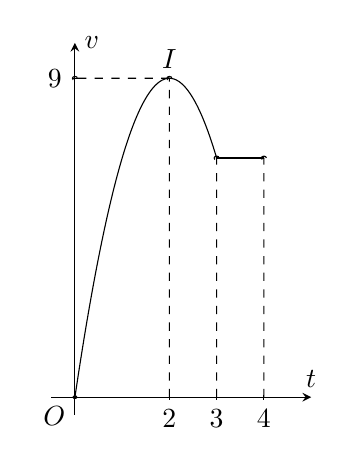
\begin{tikzpicture}[>=stealth,yscale=0.45,xscale=.6]
         % Vẽ 2 trục, điền các số lên trục
         \draw[->] (-0.5,0)--(0,0) node[below left]{$O$}--(5,0) node[above]{$t$};
         \foreach \x in {2,3,4}
         \draw[shift={(\x,0)},color=black] (0pt,2pt)--(0pt,-2pt) 
         node[below] { $\x$};
         \draw[->] (0,-0.5)--(0,10) node[right]{$v$};
         \foreach \y in {9}
         \draw[shift={(0,\y)}] (2pt,0pt) -- (-2pt,0pt) 
         node[left] {$\y$};
         \clip(-1,-1) rectangle (5,10); 
         %Vẽ đồ thị
         \draw[smooth,samples=100,domain=0:3, font=\footnotesize, line join=round, line cap=round, smooth] 
         plot(\x,{(-9/4)*(\x)^2+9*(\x)});
         \draw[smooth,samples=100, font=\footnotesize, line join=round, line cap=round,  smooth,domain=3:4] 
         plot(\x,{27/4});
         % Vẽ thêm mấy cái râu ria
         \draw[dashed] (3,0)--(3,27/4) circle(1.5pt);  \draw[dashed] (2,0)--(2,9) circle(1.5pt) node[above]{$I$}--(0,9) circle(1.5pt); \draw[dashed] (4,0)--(4,27/4) circle(1.5pt);
         %Vẽ dấu chấm tròn 
         \fill (0cm,0cm) circle (1.5pt); 
     \end{tikzpicture} 
 }
% \loigiai{
% \begin{itemize}
% \item Dựa vào đồ thị, đỉnh của parabol là $I(2; 9)$ nên vận tốc lớn nhất là $v_{\max} = 9\text{ km/h}$. \textbf{Ý a) Đúng}.
% \item Gọi phương trình của parabol là $v(t) = a(t-2)^2 + 9$.
% Vì parabol đi qua gốc tọa độ $O(0;0)$ nên ta có:
% $$a(0-2)^2 + 9 = 0 \Leftrightarrow 4a = -9 \Leftrightarrow a = -\frac{9}{4}.$$
% Suy ra phương trình vận tốc trên $[0; 3]$ là $v(t) = -\frac{9}{4}(t-2)^2 + 9 = -\frac{9}{4}t^2 + 9t$. \textbf{Ý b) Đúng}.
% \item Tại thời điểm $t = 3$, vận tốc là $v(3) = -\frac{9}{4} \cdot 3^2 + 9 \cdot 3 = \frac{27}{4}$.
% Trên đoạn $[3; 4]$, đồ thị là đường thẳng song song với trục hoành nên có phương trình không đổi $v(t) = \frac{27}{4}$. \textbf{Ý c) Sai}.
% \item Quãng đường vật đi được trong $4$ giờ là:
% $$S = \int\limits_{0}^{3} \left(-\frac{9}{4}t^2 + 9t\right) \mathrm{d}t + \int\limits_{3}^{4} \frac{27}{4} \mathrm{d}t = \frac{81}{4} + \frac{27}{4} = 27 \text{ (km)}.$$
% \textbf{Ý d) Đúng}.
% \end{itemize}
% }
\end{ex}
\begin{ex}[Phan Bội Châu - Hà Tĩnh - 2025]
 \immini[thm]{Vật thể chuyển động trong $10$ phút với vận tốc là giá trị hàm số
 \[v(t)=\heva{&a{t^2}+bt+c
 \quad \left(0\le t\le 6\right)\\&
 m\quad \quad\quad \quad \quad\left(6 < t\le 10\right)}\]
 trong đó đơn vị của $v(t)$ là m/phút, đơn vị của $t$ là phút. Đồ thị của hàm số vận tốc như hình vẽ bên.}{\begin{tikzpicture}[xscale=0.3,yscale=.3]
     % Trục toạ độ
     \draw[->] (0,0) -- (12,0) node[right] {$t$(phút)};
     \draw[->] (0,0) -- (0,11) node[above] {$v(m)$};
     % Vẽ parabol: v(t) = -40t^2 + 400t, chia 100 để scale đẹp
     \draw[domain=0:6,smooth,variable=\t] 
     plot ({\t},{(-40*\t*\t + 400*\t)/100});
     % Đoạn nằm ngang từ (6,9.6) đến (10,9.6)
     \draw (6,9.6) -- (10,9.6);
     % Các đường đứt đoạn thẳng đứng
     \draw[dashed] (5,0) -- (5,10);
     \draw[dashed] (6,0) -- (6,9.6);
     \draw[dashed] (10,0) -- (10,9.6);
     \draw[dashed] (0,10) -- (5,10);
     % Ghi nhãn các mốc
     \node at (5,-0.7) {5};
     \node at (6,-0.7) {6};
     \node at (10,-0.7) {10};
     \node[left] at (-0.3,10) {1000};
     %\node at (-0.6,9.6) {960};
     \node[below] at (-0.3,0) {O};
     \end{tikzpicture}}
\choiceTF
{\True Trong khoảng từ phút thứ $ 6$ đến phút thứ $ 10$, vận tốc vật thể không thay đổi}
{\True Quãng đường đi được của vật thể sau 6 phút đầu tiên là $\displaystyle\int\limits_0^6v(t)\,\mathrm{d}t$}
{$ 5a+b=20$}
{\True Tổng quãng đường đi được của vật thể sau $ 10$ phút đầu tiên là $ 8\,160$m}
% \loigiai{
% \begin{itemchoice}
% \itemch Dựa vào hàm số $ v(t)=\heva{&a{t^2}+bt+c
% \quad \left(0\le t\le 6\right)\\&
% m\quad \quad\quad \quad \quad\left(6 < t\le 10\right)}$, ta thấy trong khoảng thời gian từ phút thứ $ 6$ đến phút thứ $ 10$, hàm số $ v(t)$ là hàm hằng nên vận tốc vật thể không thay đổi.
% \itemch Quãng đường đi được của vật thể sau 6 phút đầu tiên là $\displaystyle\int\limits_0^6v(t)\,\mathrm{d}t$.
% \itemch
% Xét trong khoảng thời gian từ phút thứ $ 6$ đến phút thứ $ 10$, hàm số $ v(t)=a{t^2}+bt+c$ có đồ thị là một phần của Parabol đỉnh $\left(5;1000\right)$ và đi qua gốc tọa độ $ O\left(0;0\right)$ nên ta có hệ phương trình
% \allowdisplaybreaks
% \begin{eqnarray*}
% \heva{&
% a\cdot{5^2}+b\cdot5+c=1\,000\\&
% -\dfrac{b}{2a}=5\\&
% a{0^2}+b.0+c=0}\Leftrightarrow\heva{&25a+5b=1\,000\\&10a+b=0\\&c=0}\Leftrightarrow\heva{&a=-40\\&b=400\\&c=0.}
% \end{eqnarray*}
% Vậy $5a+b=5\left(-40\right)+400=200$.
% \itemch
% Theo câu c), trong khoảng thời gian từ phút thứ $6$ đến phút thứ $10$, ta được $v(t)=-40t^2+400t$.\\
% Tại $t=6\Rightarrow v=960$. Do đó $m=960$.\\
% Tóm lại $ v(t)=\heva{&-40t^2+400t\quad\left(0\le t\le 6\right)\\&960\quad\quad\quad\quad\quad\quad\left(6 < t\le 10\right)}$.\\
% Vậy tổng quãng đường đi được của vật thể sau $ 10$ phút đầu tiên là\\
% $$ s=\displaystyle\int\limits_0^6\left(-40t^2+400t\right)\,\mathrm{d}t+\displaystyle\int\limits_6^{10}960\,\mathrm{d}t=8\,160\text{m}$$.
% \end{itemchoice}
% }
 
\end{ex}
\begin{ex}[Chuyên KHTN Lần 2-Hà Nội-2026]
    \immini[thm]{Cho đồ thị biểu diễn vận tốc của hai xe A và B khởi hành cùng một lúc, bên cạnh nhau và trên cùng một con đường. Biết đồ thị biểu diễn vận tốc của xe A là $v_A(t)$ (km/h) một đường parabol, đồ thị biểu diễn vận tốc của xe B là một đường thẳng $v_B(t)$ (km/h) ở hình bên.
        \choiceTF
        {Phương trình vận tốc của xe B là $v_B(t) = 15t$}
        {\True Vận tốc lớn nhất của xe A trong 4 giờ đầu di chuyển là 80 km/h}
        {Quãng đường xe A đi được trong 3 giờ đầu là 120 km}
        {Khoảng cách hai xe lớn nhất trong 4 giờ đầu là $\frac{160}{3}$ km}}{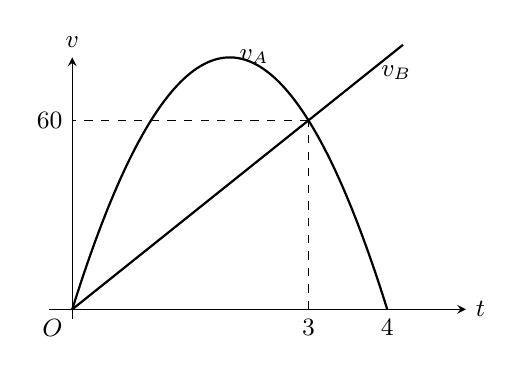
\begin{tikzpicture}[>=stealth, font=\small, x=1cm, y=0.04cm]
            % Draw axes with arrows
            \draw[->] (-0.3,0) -- (5.0,0) node[right] {$t$};
            \draw[->] (0,-3) -- (0,80) node[above] {$v$};
            % Label the origin
            \node[below left] at (0,0) {$O$};
            \draw[thick, samples=100, domain=0:4] plot (\x, {-20*\x*(\x-4)});
            % vB is a straight line passing through (0,0) and (3,60)
            \draw[thick, domain=0:4.2] plot (\x, {20*\x});
            % Label the curves
            \node[anchor=south west] at (2,75) {$v_A$};
            \node[anchor=south west] at (3.8, 70) {$v_B$};
            % Draw intersection lines
            \draw[dashed] (3,0) -- (3,60);
            \draw[dashed] (3,60) -- (0,60);
            % Label the key values on the axes
            \node[below] at (3,0) {$3$};
            \node[below] at (4,0) {$4$};
            \node[left] at (0,60) {$60$};
    \end{tikzpicture}}
    \loigiai{
        \textbf{Đánh giá các phát biểu:}
        \begin{itemize}
            \item \textbf{Phát biểu a) Sai.} Dựa vào đồ thị, đường thẳng $v_B(t)$ đi qua gốc tọa độ $O(0;0)$ và điểm $(3; 60)$. Do đó hệ số góc của đường thẳng là $k = \frac{60}{3} = 20$. Phương trình vận tốc của xe B là $v_B(t) = 20t$.
            \item \textbf{Phát biểu b) Đúng.} Parabol $v_A(t) = at^2 + bt + c$ đi qua các điểm $(0;0)$, $(4;0)$ và $(3;60)$. 
            Ta có hệ phương trình:
            $$ \begin{cases} c = 0 \\ 16a + 4b = 0 \\ 9a + 3b = 60 \end{cases} \Leftrightarrow \begin{cases} b = -4a \\ 9a - 12a = 60 \\ c = 0 \end{cases} \Leftrightarrow \begin{cases} a = -20 \\ b = 80 \\ c = 0 \end{cases} $$
            Vậy $v_A(t) = -20t^2 + 80t$. 
            Đỉnh của parabol đạt tại $t = -\frac{b}{2a} = 2$. Vận tốc lớn nhất của xe A là $v_A(2) = -20(2)^2 + 80(2) = 80$ (km/h).
            \item \textbf{Phát biểu c) Sai.} Quãng đường xe A đi được trong 3 giờ đầu là tích phân của vận tốc:
            $$ S_A = \int_{0}^{3} (-20t^2 + 80t) dt = \left[ -\frac{20}{3}t^3 + 40t^2 \right]_{0}^{3} = -180 + 360 = 180 \text{ (km)} $$
            \item \textbf{Phát biểu d) Sai.} Hàm biểu diễn khoảng cách giữa hai xe trong 4 giờ đầu là $h(t) = |S_A(t) - S_B(t)|$.
            Ta xét hiệu quãng đường (do xe A đi nhanh hơn trong 3 giờ đầu):
            $$ f(t) = S_A(t) - S_B(t) = \int_{0}^{t} (v_A(x) - v_B(x)) dx = \int_{0}^{t} (-20x^2 + 60x) dx = -\frac{20}{3}t^3 + 30t^2 $$
            Khảo sát hàm $f(t)$ trên đoạn $[0; 4]$:
            $$ f'(t) = -20t^2 + 60t = 0 \Leftrightarrow \left[ \begin{array}{l} t = 0 \\ t = 3 \end{array} \right. $$
            Ta có $f(0) = 0$, $f(3) = 90$, $f(4) = \frac{160}{3} \approx 53,33$.
            Vậy khoảng cách lớn nhất giữa hai xe là 90 km (đạt được tại thời điểm $t = 3$ giờ).
        \end{itemize}
    }
      \dotlineEX{3}
\end{ex}
\begin{ex}
 \immini[thm]{Ở Dubai, những hòn đảo nhân tạo được xây dựng trên biển để làm địa điểm nghỉ dưỡng. Trên hệ tọa độ $Oxy$, đơn vị mỗi trục tính bằng $100$ mét, đường bờ biển của một hòn đảo được mô tả như hình vẽ bởi các đồ thị hàm số $y = f(x)$ và $y = g(x)$. Trong đó $y = f(x)$ là một parabol có đỉnh $I(4; 2)$, đi qua gốc tọa độ và $g(x) = (2x - 20)\mathrm{e}^{0{,}2x - 2}$. Hòn đảo này gồm hai phần: phần bãi tắm được giới hạn bởi đường cong $y = f(x)$ và trục hoành; phần nghỉ dưỡng được giới hạn bởi đường cong $y = g(x)$, trục tung và trục hoành (tham khảo hình vẽ).
 }{\includegraphics[scale=.2]{images/2.22}}
 \choiceTF
 {\True $f(x) = -0{,}125x^2 + x$}
 {\True Diện tích của bãi tắm lớn hơn $100$ nghìn mét vuông}
 {Biết rằng $G(x) = (ax + b)\mathrm{e}^{0{,}2x - 2}$ là một nguyên hàm của hàm số $g(x)$ trên $\mathbb{R}$, khi đó $a - b = 140$}
 {Tổng diện tích hòn đảo lớn hơn $500$ nghìn mét vuông}
 \loigiai{a) Gọi phương trình parabol là $f(x) = ax^2+bx+c$. Đỉnh $I(4; 2)$ và parabol đi qua gốc tọa độ $O(0;0)$ nên ta có hệ:$\begin{cases} c=0 \\ -\dfrac{b}{2a} = 4 \\ 16a + 4b + c = 2 \end{cases} \Leftrightarrow \begin{cases} c=0 \\ b = -8a \\ 16a - 32a = 2 \end{cases} \Leftrightarrow \begin{cases} a = -0{,}125 \\ b = 1 \\ c = 0 \end{cases}$.Vậy $f(x) = -0{,}125x^2 + x$. $\Rightarrow$ Mệnh đề a) Đúng.b) Phương trình hoành độ giao điểm của đường cong bãi tắm với trục hoành:$-0{,}125x^2 + x = 0 \Leftrightarrow x=0$ hoặc $x=8$.Diện tích bãi tắm trên mặt phẳng tọa độ:$S_1 = \displaystyle\int\limits_0^8 \left(-0{,}125x^2 + x\right) \mathrm{d}x = \dfrac{32}{3}$.Do $1$ đơn vị trên trục bằng $100\text{ m}$ nên $1$ đvdt $= 100 \times 100 = 10\,000\text{ m}^2$.Diện tích bãi tắm thực tế: $S_{\text{bãi tắm}} = \dfrac{32}{3} \times 10\,000 \approx 106\,667\text{ m}^2 > 100\,000\text{ m}^2$. $\Rightarrow$ Mệnh đề b) Đúng.c) Ta có $G'(x) = a\mathrm{e}^{0{,}2x-2} + 0{,}2(ax+b)\mathrm{e}^{0{,}2x-2} = (0{,}2ax + a + 0{,}2b)\mathrm{e}^{0{,}2x-2}$.Để $G(x)$ là nguyên hàm của $g(x)$ thì $G'(x) = g(x) = (2x - 20)\mathrm{e}^{0{,}2x - 2}$, đồng nhất hệ số ta được:$\begin{cases} 0{,}2a = 2 \\ a + 0{,}2b = -20 \end{cases} \Leftrightarrow \begin{cases} a = 10 \\ 10 + 0{,}2b = -20 \end{cases} \Leftrightarrow \begin{cases} a = 10 \\ b = -150 \end{cases}$.Khi đó $a - b = 10 - (-150) = 160 \neq 140$. $\Rightarrow$ Mệnh đề c) Sai.d) Giao điểm của $y=g(x)$ với trục hoành: $(2x - 20)\mathrm{e}^{0{,}2x - 2} = 0 \Leftrightarrow x = 10$.Diện tích phần nghỉ dưỡng trên mặt phẳng tọa độ:$S_2 = \displaystyle\int\limits_0^{10} \left|g(x)\right| \mathrm{d}x = \displaystyle\int\limits_0^{10} -(2x - 20)\mathrm{e}^{0{,}2x - 2} \mathrm{d}x = -\left. G(x) \right|_0^{10}$.Với $G(x) = (10x - 150)\mathrm{e}^{0{,}2x - 2}$, ta có:$S_2 = -\left[ (100 - 150)\mathrm{e}^0 - (-150)\mathrm{e}^{-2} \right] = 50 - 150\mathrm{e}^{-2} \approx 29{,}70$.Tổng diện tích hòn đảo trên mặt phẳng tọa độ:$S = S_1 + S_2 = \dfrac{32}{3} + 50 - 150\mathrm{e}^{-2} \approx 40{,}37$.Tổng diện tích hòn đảo thực tế: $S_{\text{tổng}} = S \times 10\,000 \approx 403\,700\text{ m}^2 < 500\,000\text{ m}^2$. $\Rightarrow$ Mệnh đề d) Sai.}
   \dotlineEX{5}
\end{ex}
\begin{ex}
 \immini[thm]{Cho hàm số $f(x)$ liên tục trên đoạn $[-1;6]$ và có đồ thị hình gấp khúc $ABC$ trong hình bên. Biết $F(x)$ là nguyên hàm của $f(x)$ trên $\mathbb{R}$ thỏa mãn $F(-1)=-1$. Giá trị của $F(5)+F(6)$ bằng
 \shortans{$19$}}{\includegraphics[width=4cm]{images/2.12}}
% \loigiai{
% Dựa vào đồ thị ta thấy:
% Diện tích hình phẳng phần nằm trên trục hoành (giới hạn bởi đồ thị $f(x)$, trục hoành và các đường thẳng $x=-1$, $x=5$) là:
% $$S_1 = S_{HCN} + S_{\Delta 1} = 5 \cdot 2 + \frac{1}{2} \cdot 1 \cdot 2 = 11.$$
% Do đó $\int\limits_{-1}^{5} f(x) \mathrm{d}x = 11$.
% Mà $\int\limits_{-1}^{5} f(x) \mathrm{d}x = F(5) - F(-1) \Rightarrow F(5) - (-1) = 11 \Leftrightarrow F(5) = 10$.
% Diện tích hình phẳng phần nằm dưới trục hoành (giới hạn bởi đồ thị $f(x)$, trục hoành và các đường thẳng $x=5$, $x=6$) là:
% $$S_2 = \frac{1}{2} \cdot 1 \cdot 2 = 1.$$
% Do phần này nằm dưới trục hoành nên $\int\limits_{5}^{6} f(x) \mathrm{d}x = -1$.
% Mà $\int\limits_{5}^{6} f(x) \mathrm{d}x = F(6) - F(5) \Rightarrow F(6) - 10 = -1 \Leftrightarrow F(6) = 9$.
% Vậy $F(5)+F(6) = 10 + 9 = 19$.
% }
\dotlineEX{2}
\end{ex}
\begin{ex}
 \immini[thm]{Cho hàm số $f(x)$. Đồ thị hàm số $y=f'(x)$ trên đoạn $[-3;0]$ như hình vẽ sau (phần đường cong trong đồ thị là một phần của parabol $y=ax^2+bx+c$). Biết $f(0)=-\frac{2}{3}$, tính $f(-3)$.
 \shortans{$-3$}}{\includegraphics[width=4cm]{images/2.13}}
% \loigiai{
% Dựa vào đồ thị $f'(x)$, ta có:
% Trên đoạn $[-3;-1]$, đồ thị là một phần của parabol có đỉnh $(-2;1)$ và đi qua điểm $(-1;0)$ nên phương trình parabol có dạng $y = a(x+2)^2+1$.
% Vì parabol đi qua $(-1;0)$ nên $a(-1+2)^2+1 = 0 \Leftrightarrow a = -1$.
% Suy ra trên $[-3;-1]$, ta có $f'(x) = -(x+2)^2+1 = -x^2-4x-3$.
% Trên đoạn $[-1;0]$, đồ thị là đoạn thẳng đi qua hai điểm $(-1;0)$ và $(0;2)$ nên có phương trình $y = 2x+2$.
% Suy ra trên $[-1;0]$, ta có $f'(x) = 2x+2$.
% Ta có: $\int\limits_{-3}^{0} f'(x) \mathrm{d}x = \int\limits_{-3}^{-1} f'(x) \mathrm{d}x + \int\limits_{-1}^{0} f'(x) \mathrm{d}x = \int\limits_{-3}^{-1} (-x^2-4x-3) \mathrm{d}x + \int\limits_{-1}^{0} (2x+2) \mathrm{d}x$.
% Tính các tích phân:
% $$ \int\limits_{-3}^{-1} (-x^2-4x-3) \mathrm{d}x = \left( -\frac{x^3}{3} - 2x^2 - 3x \right)\Bigg|_{-3}^{-1} = \frac{4}{3} - 0 = \frac{4}{3}. $$
% $$ \int\limits_{-1}^{0} (2x+2) \mathrm{d}x = \left( x^2+2x \right)\Bigg|_{-1}^{0} = 0 - (-1) = 1. $$
% Vậy $\int\limits_{-3}^{0} f'(x) \mathrm{d}x = \frac{4}{3} + 1 = \frac{7}{3}$.
% Mặt khác $\int\limits_{-3}^{0} f'(x) \mathrm{d}x = f(0) - f(-3) \Rightarrow \frac{7}{3} = -\frac{2}{3} - f(-3) \Rightarrow f(-3) = -\frac{2}{3} - \frac{7}{3} = -3$.
% }
\dotlineEX{2}
\end{ex}
\begin{ex}
    \immini[thm]{ Cho $S_1$, $S_2$ là diện tích các hình phẳng được mô tả trong hình vẽ bên. Biết tỉ số $\frac{S_1}{S_2} = \frac{a}{b}$ ($a, b \in \mathbb{N}^*$) và phân số $\frac{a}{b}$ tối giản, tính tổng $a+b$.
        \shortans{$64$}}{
        \begin{tikzpicture}[>=stealth,scale=.8]
            \def\f(#1){-(#1)^2+4(#1)}
            \fill[pattern=north west lines, opacity=0.5]
            plot[domain=0:3](\x,{-(\x)^2+4*(\x)}) -- plot[domain=0:3](\x,{\x})--cycle;
            \fill[pattern=dots, opacity=0.5]
            plot[domain=3:4](\x,{-(\x)^2+4*(\x)}) -- plot[domain=0:4](\x,{\x})--cycle;
            \draw[->](-.5,0)--(5,0)node[above]{$x$};
            \draw[->](0,-.5)--(0,4.5)node[below right]{$y$};
            \path 
            (0,0) node[below right]{$0$};
            \draw[dashed] (0,3)--(3,3) (3,0)--(3,3) ;
            \draw
            (4,3.8) node[below]{$(d)$}
            (4.5,1.5) node[below left]{$(P)$}
            (3,0) node[below]{$3$}
            (4,0) node[below right]{$4$}
            (0,3) node[left]{$3$}
            (2,2.5) node[left]{$S_1$}
            (2,1.5) node[right]{$S_2$};
            \draw[,samples=100]
            plot[domain=-.4:4](\x,{\x});
            \draw[,samples=100]
            plot[domain=-.1:4.1](\x,{4*\x-(\x)^2});
        \end{tikzpicture}
    }
%    \loigiai{
%        Phương trình hoành độ giao điểm của parabol $y = -x^2+4x$ và đường thẳng $y=x$:
%        $$-x^2+4x = x \Leftrightarrow -x^2+3x = 0 \Leftrightarrow \hoac{&x=0\\&x=3.}$$
%        Diện tích $S_1$ (phần hình phẳng giới hạn bởi parabol và đường thẳng trên đoạn $[0;3]$) là:
%        $$S_1 = \int\limits_0^3 \left( -x^2+4x - x \right) \mathrm{d}x = \int\limits_0^3 \left( -x^2+3x \right) \mathrm{d}x = \left( -\frac{x^3}{3} + \frac{3x^2}{2} \right)\Bigg|_0^3 = \frac{9}{2}.$$
%        Tổng diện tích $S$ giới hạn bởi parabol và trục hoành trên đoạn $[0;4]$ là:
%        $$S = \int\limits_0^4 \left( -x^2+4x \right) \mathrm{d}x = \left( -\frac{x^3}{3} + 2x^2 \right)\Bigg|_0^4 = \frac{32}{3}.$$
%        Phần diện tích $S_2$ là: $S_2 = S - S_1 = \frac{32}{3} - \frac{9}{2} = \frac{37}{6}$.
%        Tỉ số $\frac{S_1}{S_2} = \frac{9/2}{37/6} = \frac{27}{37}$.
%        Vì $\frac{a}{b}$ là phân số tối giản nên $a=27, b=37$.
%        Vậy tổng $a+b = 27 + 37 = 64$.
%    }
\dotlineEX{2}
\end{ex}
\begin{ex}
 \immini[thm]{ Cho hàm số $y = f(x) = ax^2+1$, $y=2$ có đồ thị như hình vẽ. Gọi $S_1, S_2$ là các diện tích hình phẳng trong hình bên. Biết rằng $S_1 = S_2$, tính diện tích $S_1$. Viết kết quả làm tròn đến hàng phần trăm.
 \shortans{$1,15$}}{ \includegraphics[width=4cm]{images/2.15}}
% \loigiai{
% Phương trình hoành độ giao điểm của $y = ax^2+1$ và $y=2$ (với $x>0$):
% $$ax^2+1 = 2 \Leftrightarrow x^2 = \frac{1}{a} \Rightarrow x = \frac{1}{\sqrt{a}}.$$
% Diện tích $S_1$ là:
% $$S_1 = \int\limits_0^{\frac{1}{\sqrt{a}}} \left[ 2 - (ax^2+1) \right] \mathrm{d}x = \int\limits_0^{\frac{1}{\sqrt{a}}} (1 - ax^2) \mathrm{d}x = \left( x - \frac{ax^3}{3} \right)\Bigg|_0^{\frac{1}{\sqrt{a}}} = \frac{1}{\sqrt{a}} - \frac{1}{3\sqrt{a}} = \frac{2}{3\sqrt{a}}.$$
% Diện tích $S_2$ là:
% $$S_2 = \int\limits_{\frac{1}{\sqrt{a}}}^3 \left[ (ax^2+1) - 2 \right] \mathrm{d}x = \int\limits_{\frac{1}{\sqrt{a}}}^3 (ax^2-1) \mathrm{d}x = \left( \frac{ax^3}{3} - x \right)\Bigg|_{\frac{1}{\sqrt{a}}}^3 = (9a-3) - \left( \frac{1}{3\sqrt{a}} - \frac{1}{\sqrt{a}} \right) = 9a - 3 + \frac{2}{3\sqrt{a}}.$$
% Theo giả thiết $S_1 = S_2$, ta có:
% $$\frac{2}{3\sqrt{a}} = 9a - 3 + \frac{2}{3\sqrt{a}} \Leftrightarrow 9a - 3 = 0 \Leftrightarrow a = \frac{1}{3}.$$
% Suy ra $S_1 = \frac{2}{3\sqrt{1/3}} = \frac{2\sqrt{3}}{3} \approx 1.1547$.
% Làm tròn đến hàng phần trăm, ta được $1.15$.
% }
\end{ex}
\begin{ex}[KCSL12-Sở Hà Nội-2026]
 \immini[thm]{Trong lưới ô vuông có hai đường parabol như hình vẽ. Biết rằng mỗi ô vuông nhỏ có cạnh bằng $1\text{ cm}$. Diện tích của hình phẳng trong lưới ô vuông được giới hạn bởi hai đường parabol (phần tô màu) bằng bao nhiêu centimet vuông (kết quả làm tròn đến hàng phần trăm)?
 \shortans{9,76}}{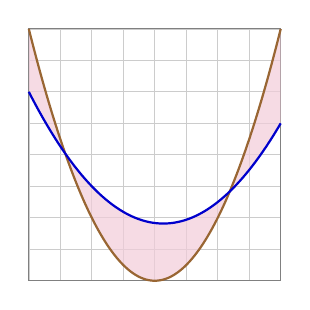
\begin{tikzpicture}[scale=0.4, >=stealth]
 % Lưới ô vuông 8x8
 \draw[step=1cm, gray!40, very thin] (-4,0) grid (4,8);
 \draw[gray, thin] (-4,0) rectangle (4,8);
 % Tô màu phần gạch chéo
 % x1 ~ -2.8427, x2 ~ 2.3812
 \fill[purple!20, opacity=0.7] plot[domain=-4:-2.8427, samples=50] (\x, {0.5*\x*\x}) -- plot[domain=-2.8427:-4, samples=50] (\x, {11/48*\x*\x - 1/8*\x + 11/6}) -- cycle;
 \fill[purple!20, opacity=0.7] plot[domain=-2.8427:2.3812, samples=50] (\x, {11/48*\x*\x - 1/8*\x + 11/6}) -- plot[domain=2.3812:-2.8427, samples=50] (\x, {0.5*\x*\x}) -- cycle;
 \fill[purple!20, opacity=0.7] plot[domain=2.3812:4, samples=50] (\x, {0.5*\x*\x}) -- plot[domain=4:2.3812, samples=50] (\x, {11/48*\x*\x - 1/8*\x + 11/6}) -- cycle;
 % Vẽ hai parabol
 \draw[brown!80!black, thick, smooth, domain=-4:4, samples=100] plot (\x, {0.5*\x*\x});
 \draw[blue!80!black, thick, smooth, domain=-4:4, samples=100] plot (\x, {11/48*\x*\x - 1/8*\x + 11/6});
 \end{tikzpicture}} 
% \loigiai{
% Chọn hệ trục tọa độ $Oxy$ sao cho gốc tọa độ $O$ trùng với đỉnh của parabol hướng bề lõm lên trên (parabol màu nâu). 
% \begin{itemize}
% \item Parabol thứ nhất $(P_1)$ là $y_1 = \frac{1}{2}x^2$.
% \item Parabol thứ hai $(P_2)$ là $y_2 = \frac{11}{48}x^2 - \frac{1}{8}x + \frac{11}{6}$.
% \end{itemize}
% Diện tích phần gạch chéo cần tìm là diện tích hình phẳng giới hạn bởi $(P_1)$ và $(P_2)$ trên đoạn $[-4; 4]$:
% $$S = \int_{-4}^{4} \left| -\frac{13}{48}x^2 - \frac{1}{8}x + \frac{11}{6} \right| \mathrm{d}x$$
% Sử dụng máy tính cầm tay để tính tích phân trên, ta được kết quả:
% $$S \approx 9{,}76\ (\text{cm}^2).$$
% }
\dotlineEX{3}
\end{ex}
\begin{ex}[KSCL12-Sở Hà Nội-2025]%[Câu 27]
 \immini[thm]{ Một cửa vòm có dạng hình parabol được lắp các tấm kính hình tròn đường kính $1\text{m}$ và các tấm kính hình vuông có cạnh $1\text{m}$ như hình vẽ. Phần còn lại của cửa được sơn màu trang trí với mức giá $1,2$ triệu đồng $/ \text{m}^2$. Chi phí sơn màu là bao nhiêu triệu đồng (kết quả làm tròn đến hàng phần chục)?
 \shortans{$8,1$}}{\includegraphics[scale=.3]{images/2.17}}
 \loigiai{
 Chọn hệ trục tọa độ $Oxy$ như hình vẽ, với gốc $O$ là trung điểm của đoạn thẳng $AB$, trục tung $Oy$ là trục đối xứng của vòm.
 Dựa vào kích thước của đường tròn đường kính $1$ và hình vuông cạnh $1$, ta xác định được:
 \begin{itemize}
 \item Đỉnh vòm $P$ nằm trên trục $Oy$ có tung độ $OP = 4 \Rightarrow P(0; 4)$.
 \item Khối kính hình vuông có bề ngang lớn nhất (đoạn $MN$) bằng $4$ (gồm 4 hình vuông) và mép trên của khối này cách mặt đất một khoảng bằng $2$. Do đó $M(-2; 2)$ và $N(2; 2)$.
 \end{itemize}
 Vì parabol đi qua các điểm $P, M, N$ nên giả sử phương trình parabol có dạng $y = ax^2 + c$.
 Vì parabol có đỉnh $P(0; 4)$ nên $c = 4 \Rightarrow y = ax^2 + 4$.
 Parabol đi qua $N(2; 2)$ nên ta có:
 $$a \cdot 2^2 + 4 = 2 \Leftrightarrow 4a = -2 \Leftrightarrow a = -\frac{1}{2}.$$
 Vậy phương trình parabol là $y = -\frac{1}{2}x^2 + 4$.
 Hoành độ các điểm $A, B$ tại chân vòm là nghiệm của phương trình:
 $$-\frac{1}{2}x^2 + 4 = 0 \Leftrightarrow x^2 = 8 \Leftrightarrow x = \pm 2\sqrt{2}.$$
 Suy ra $A(-2\sqrt{2}; 0)$ và $B(2\sqrt{2}; 0)$.
 Tổng diện tích các tấm kính là:
 $$S_1 = 3 \cdot \pi \cdot (0,5)^2 + 6 \cdot 1 \cdot 1 = 0,75\pi + 6 \text{ (m}^2\text{)}.$$
 Diện tích toàn bộ cửa vòm (phần giới hạn bởi parabol và trục $Ox$) là:
 $$S = \int\limits_{-2\sqrt{2}}^{2\sqrt{2}} \left( -\frac{1}{2}x^2 + 4 \right) \mathrm{d}x = \left( -\frac{x^3}{6} + 4x \right)\Bigg|_{-2\sqrt{2}}^{2\sqrt{2}} = \frac{32\sqrt{2}}{3} \text{ (m}^2\text{)}.$$
 Chi phí sơn màu phần còn lại là:
 $$T = 1,2 \cdot (S - S_1) = 1,2 \cdot \left( \frac{32\sqrt{2}}{3} - 0,75\pi - 6 \right) \approx 8,074 \text{ (triệu đồng)}.$$
 Làm tròn đến hàng phần chục, ta được kết quả là $8,1$ triệu đồng.
 }
 \dotlineEX{2}
\end{ex}
\begin{ex}
 Mặt trong của một hầm biogas có hình dạng là một phần của mặt cầu đã cắt bỏ hai phần của nó bằng hai mặt phẳng song song với nhau (như hình vẽ). Bán kính của mặt cầu bằng $2{,}5 \mathrm{~m}$. Mặt đáy phía dưới cách tâm một khoảng bằng $1{,}5 \mathrm{~m}$. Mặt đáy phía trên cách tâm một khoảng bằng $2 \mathrm{~m}$. Thể tích gần đúng phần bên trong của hầm biogas đó bằng bao nhiêu (đơn vị là $\mathrm{m}^3$ và kết quả làm tròn đến hàng phần mười)?
 \shortans{56{,}8}
 \begin{center}
 \includegraphics[scale=0.4]{images/2.18}
 \end{center}
% \loigiai{
% Trên hệ trục $Oxy$ xét đường tròn $(C)$ có phương trình $x^2 + y^2 = 2{,}5^2$. Khi đó nửa phần trên trục hoành của $(C)$ có phương trình $y = \sqrt{2{,}5^2 - x^2}$. Xét hình phẳng $(H)$ giới hạn bởi nửa phần trên trục hoành của $(C)$, trục $Ox$ và các đường thẳng $x = -1{,}5$; $x = 2$.
% Quay hình phẳng $(H)$ quanh trục hoành ta được khối tròn xoay có thể tích bằng thể tích phần không gian phía trong của hầm biogas.
% Thể tích phần không gian bên trong hầm biogas được tính bởi công thức:
% \[
% V = \pi \int\limits_{-1{,}5}^{2} \left( 2{,}5^2 - x^2 \right) \mathrm{d}x = \frac{217}{12}\pi \approx 56{,}8
% \]
% }
\dotlineEX{2}
\end{ex}
\begin{ex}[Chuyên KHTN Lần 2-Hà Nội-2026]
 Trên mặt phẳng vẽ hai nửa đường tròn đường kính $AB$, $AD$, với $AB = 2AD = 4\text{ cm}$ như hình vẽ. Cho biết $\widehat{BAC} = 30^\circ$. Hình phẳng (H) là phần tô đậm nằm giữa hai nửa đường tròn, đường thẳng $AB, AC$. Một kỹ sư cần chế tạo chi tiết máy bằng thép có dạng tròn xoay khi xoay hình phẳng (H) quanh trục $AB$. Biết chi phí sản xuất là 15 nghìn đồng/$\text{cm}^3$. Giá tiền sản xuất một chi tiết máy là bao nhiêu nghìn đồng? (kết quả làm tròn đến hàng đơn vị)
 \shortans{192}
 \begin{center}
 \includegraphics[scale=.25]{images/2.26}
 \end{center}
% \loigiai{
% Gắn hệ trục tọa độ $Oxy$ sao cho gốc tọa độ $O$ trùng với điểm $A$, tia $Ox$ trùng với tia $AB$.
% Khi đó ta có các điểm $A(0;0)$, $D(2;0)$, $B(4;0)$.
% \begin{itemize}
% \item Nửa đường tròn lớn có tâm $I_1(2;0)$, bán kính $R=2$, phương trình phần đồ thị phía trên trục hoành là $y = \sqrt{4 - (x-2)^2} = \sqrt{4x - x^2}$.
% \item Nửa đường tròn nhỏ có tâm $I_2(1;0)$, bán kính $r=1$, phương trình phần đồ thị phía trên trục hoành là $y = \sqrt{1 - (x-1)^2} = \sqrt{2x - x^2}$.
% \item Đường thẳng $AC$ đi qua gốc tọa độ, tạo với trục hoành góc $30^\circ$ nên có phương trình $y = x \cdot \tan 30^\circ = \frac{x}{\sqrt{3}}$.
% \end{itemize}
% Xác định hoành độ các giao điểm:
% \begin{itemize}
% \item Giao điểm của đường thẳng $AC$ và nửa đường tròn nhỏ: $\frac{x}{\sqrt{3}} = \sqrt{2x - x^2} \Rightarrow \frac{x^2}{3} = 2x - x^2 \Rightarrow x = 1,5$ (nhận nghiệm dương).
% \item Giao điểm của đường thẳng $AC$ và nửa đường tròn lớn: $\frac{x}{\sqrt{3}} = \sqrt{4x - x^2} \Rightarrow \frac{x^2}{3} = 4x - x^2 \Rightarrow x = 3$ (nhận nghiệm dương).
% \end{itemize}
% Hình phẳng (H) chiếu xuống trục $Ox$ được chia làm 3 miền để tính thể tích khối tròn xoay:
% \begin{itemize}
% \item $x \in [1,5; 2]$: giới hạn bởi $y = \frac{x}{\sqrt{3}}$ và $y = \sqrt{2x - x^2}$.
% \item $x \in [2; 3]$: giới hạn bởi $y = \frac{x}{\sqrt{3}}$ và trục $Ox$ ($y = 0$).
% \item $x \in [3; 4]$: giới hạn bởi $y = \sqrt{4x - x^2}$ và trục $Ox$ ($y = 0$).
% \end{itemize}
% Thể tích khối tròn xoay cần tìm là:
% $$ V = \pi \int_{1,5}^{2} \left[ \left(\frac{x}{\sqrt{3}}\right)^2 - (\sqrt{2x - x^2})^2 \right] dx + \pi \int_{2}^{3} \left(\frac{x}{\sqrt{3}}\right)^2 dx + \pi \int_{3}^{4} (\sqrt{4x - x^2})^2 dx $$
% $$ V = \pi \int_{1,5}^{2} \left( \frac{4x^2}{3} - 2x \right) dx + \pi \int_{2}^{3} \frac{x^2}{3} dx + \pi \int_{3}^{4} (4x - x^2) dx $$
% $$ V = \pi \left[ \frac{4x^3}{9} - x^2 \right]_{1,5}^{2} + \pi \left[ \frac{x^3}{9} \right]_{2}^{3} + \pi \left[ 2x^2 - \frac{x^3}{3} \right]_{3}^{4} $$
% Tính toán các giá trị:
% $$ V = \pi \left( \frac{11}{36} \right) + \pi \left( \frac{19}{9} \right) + \pi \left( \frac{5}{3} \right) = \pi \left( \frac{11 + 76 + 60}{36} \right) = \frac{147\pi}{36} = \frac{49\pi}{12} \text{ (cm}^3\text{)} $$
% Chi phí sản xuất một chi tiết máy là:
% $$ \text{Chi phí} = V \times 15 = \frac{49\pi}{12} \times 15 = \frac{245\pi}{4} \approx 192,42 \text{ (nghìn đồng)} $$
% Làm tròn đến hàng đơn vị ta được 192 nghìn đồng.
% }
\dotlineEX{3}
\end{ex}
\begin{ex}
 Hình elip được ứng dụng nhiều trong thực tiễn, đặc biệt là kiến trúc, xây dựng, thiết bị nội thất,... Mặt trong (lọt lòng) và ngoài (phủ bì) của một bồn rửa (lavabo) bằng sứ có hình dạng là một nửa khối tròn xoay khi quay quanh một trục của 2 elip có chung các trục đối xứng (hình minh họa). Thông số kỹ thuật mặt trên của bồn rửa: dài $\times$ rộng là $660 \times 380$ mm (phủ bì) và elip (lọt lòng) có trục lớn, trục nhỏ ít hơn elip phủ bì một khoảng $40$ mm. Tính thể tích chứa nước của bồn rửa (Đơn vị: lít và làm tròn kết quả đến hàng phần mười). \shortans{18,8}
 \begin{center}
 \includegraphics[scale=.5]{images/2.20}
 \end{center}
 \loigiai{
 Chọn hệ trục tọa độ $Oxy$ thích hợp với đơn vị trên trục là decimet (dm).
 Đổi đơn vị: $660$ mm $= 6,6$ dm; $380$ mm $= 3,8$ dm; $40$ mm $= 0,4$ dm.
 Kích thước trục lớn và trục nhỏ của elip lọt lòng lần lượt là:
 $2a = 6,6 - 0,4 = 6,2 \Rightarrow a = 3,1$ (dm).
 $2b = 3,8 - 0,4 = 3,4 \Rightarrow b = 1,7$ (dm).
 Phương trình elip lọt lòng: $(E): \frac{x^2}{3,1^2} + \frac{y^2}{1,7^2} = 1 \Leftrightarrow y = \pm 1,7 \sqrt{1 - \frac{x^2}{3,1^2}}$.
 Thể tích chứa nước của bồn rửa (là nửa khối tròn xoay):
 $$V = \frac{1}{2} \cdot \pi \int_{-3,1}^{3,1} 1,7^2 \left( 1 - \frac{x^2}{3,1^2} \right) \text{d}x \approx 18,8 \text{ lít.}$$
 \textbf{Trả lời: 18,8}
 }
\end{ex}
\begin{ex}
 \immini[thm]{ Một khu vườn dạng hình tròn có hai đường kính $AB, CD$ vuông góc với nhau, $AB = 12\text{m}$. Người ta làm một hồ cá có dạng hình elip với bốn đỉnh $M, N, M', N'$ như hình vẽ, biết $MN = 10\text{m}$, $M'N' = 8\text{m}$, $PQ = 8\text{m}$. Diện tích phần trồng cỏ (phần gạch sọc) bằng bao nhiêu? (đơn vị mét vuông, kết quả làm tròn đến hàng đơn vị)
 \shortans{32}}{\includegraphics[scale=.45]{images/2.19}}
 \loigiai{
 \textbf{Trả lời: 32}
 Gọi $AB$ giao $CD$ tại $O$, đặt hệ trục tọa độ $Oxy$ như hình vẽ.
 Khi đó, ta có phương trình đường tròn tâm $O$, đường kính $AB = 12\text{m}$ (bán kính $R = 6\text{m}$) là: 
 $$x^2 + y^2 = 6^2 \Rightarrow y = \pm \sqrt{6^2 - x^2}$$
 Hồ cá hình elip có độ dài trục lớn $MN = 10\text{m} \Rightarrow a = 5$, độ dài trục nhỏ $M'N' = 8\text{m} \Rightarrow b = 4$. Phương trình elip là:
 $$\frac{x^2}{25} + \frac{y^2}{16} = 1 \Rightarrow y = \pm 4 \sqrt{1 - \frac{x^2}{25}}$$
 Ta thấy phần trồng cỏ chia thành 2 phần bằng nhau (đối xứng qua trục $Ox$). Gọi diện tích phần phía trên trục $Ox$ là $S_1$.
 Dựa vào giả thiết $PQ = 8\text{m}$ và tính đối xứng, giới hạn tích phân sẽ đi từ $-4$ đến $4$.
 Diện tích $S_1$ được tính bởi:
 $$S_1 = \int_{-4}^{4} \left( \sqrt{6^2 - x^2} - 4 \sqrt{1 - \frac{x^2}{25}} \right) \text{d}x$$
 Vậy tổng diện tích trồng cỏ là:
 $$S = 2S_1 \approx 32\text{ m}^2.$$
 }
\end{ex}
\begin{ex}[ĐH Vinh Lần 1-2026]
    \immini[thm]{Một cơ sở sản xuất thiết bị cứu hộ chế tạo một chiếc phao cứu sinh như hình minh họa. Khi đó, theo mặt cắt qua tâm, người ta thấy, bán kính ngoài của phao bằng $35\text{ cm}$, bán kính trong của phao bằng $25\text{ cm}$. Phao được làm từ một loại vật liệu đồng chất, có khối lượng riêng bằng $0{,}05\text{ g/cm}^3$ (coi phao là khối đặc, không có khoang rỗng bên trong). Tính khối lượng của chiếc phao (đơn vị kg), biết kết quả làm tròn đến hàng phần trăm, số $\pi$ nhận giá trị bằng $3{,}1416$.
        \shortans{0,74}}{\includegraphics[scale=.4]{images/2.21}}
    \loigiai{
        Chiếc phao cứu sinh có dạng khối tròn xoay (hình xuyến).
        Gọi $R$ là khoảng cách từ trục quay đến tâm đường tròn thiết diện ống phao, $r$ là bán kính đường tròn thiết diện ống phao.
        Theo giả thiết, ta có:
        $$ \begin{cases} R + r = 35 \\ R - r = 25 \end{cases} \Leftrightarrow \begin{cases} R = 30\text{ (cm)} \\ r = 5\text{ (cm)} \end{cases} $$
        Thể tích của chiếc phao (khối xuyến) là:
        $$ V = (2\pi R) \cdot (\pi r^2) = 2\pi^2 R r^2 = 2 \cdot \pi^2 \cdot 30 \cdot 5^2 = 1500\pi^2\text{ (cm}^3) $$
        Khối lượng của chiếc phao tính theo gam là:
        $$ m = V \cdot \rho = 1500\pi^2 \cdot 0{,}05 = 75\pi^2\text{ (g)} $$
        Đổi ra kilôgam, ta có khối lượng phao là:
        $$ m = \frac{75\pi^2}{1000} = 0{,}075\pi^2\text{ (kg)} $$
        Thay $\pi = 3{,}1416$, ta tính được:
        $$ m \approx 0{,}075 \cdot (3{,}1416)^2 \approx 0{,}74022\dots\text{ (kg)} $$
        Làm tròn kết quả đến hàng phần trăm, ta được khối lượng chiếc phao là $0{,}74\text{ kg}$.
        \textbf{Đáp số:} $0{,}74$.
    }
\end{ex}
\begin{ex}
    \immini[thm]{Một kiến trúc sư chịu trách nhiệm thiết kế một tòa nhà cao $30$ mét. Mặt cắt ngang tại mọi độ cao, vuông góc với trục thẳng đứng, luôn là một hình vuông (xem hình vẽ). Mặt đáy tòa nhà là hình vuông có cạnh $L_0 = 26 \text{ m}$, mặt đỉnh là hình vuông có cạnh $L_{30} = 20 \text{ m}$. Mặt cắt ngang tại vị trí hẹp nhất của tòa nhà: Hình vuông có cạnh $L_{min} = 13,75 \text{ m}$. Mặt cắt của tòa nhà theo mặt phẳng đứng chứa đường chéo đáy có dạng là hình phẳng giới hạn bởi hai đường cong parabol đối xứng nhau qua trục thẳng đứng đi qua tâm đáy của tòa nhà. Tính thể tích của tòa nhà đó (làm tròn đến hàng đơn vị, đơn vị tính: mét khối).
        \shortans{8976}}{\includegraphics[scale=.4]{images/2.24}}
    \loigiai{
        Chọn hệ trục tọa độ $Oxyz$ sao cho mặt đáy tòa nhà nằm trên mặt phẳng $Oxy$, trục $Oz$ là trục thẳng đứng hướng lên và đi qua tâm các mặt cắt ngang của tòa nhà. Khi đó tòa nhà nằm trong khoảng giới hạn bởi $z = 0$ đến $z = 30$.
        Mặt cắt của tòa nhà bằng mặt phẳng vuông góc với trục $Oz$ tại cao độ $z$ ($0 \le z \le 30$) là một hình vuông có độ dài cạnh là $L(z)$.
        Vì mặt cắt qua mặt phẳng chứa đường chéo đáy được giới hạn bởi các đường parabol nên độ dài đường chéo của mặt cắt ngang tại độ cao $z$ là một hàm bậc hai theo $z$. Do đó, độ dài cạnh của mặt cắt ngang $L(z)$ cũng là một hàm bậc hai theo $z$: $L(z) = az^2 + bz + c$ ($a > 0$).
        Theo giả thiết, ta có:
        \begin{itemize}
            \item Cạnh đáy $L(0) = 26 \Rightarrow c = 26$.
            \item Cạnh đỉnh $L(30) = 20 \Rightarrow a \cdot 30^2 + b \cdot 30 + 26 = 20 \Leftrightarrow 900a + 30b = -6 \Leftrightarrow b = -0,2 - 30a$.
            \item Vị trí hẹp nhất đạt tại đỉnh của parabol, có tọa độ $z_0 = -\frac{b}{2a}$.
        \end{itemize}
        Tại đây, cạnh hình vuông đạt giá trị nhỏ nhất:
        $$L\left(-\frac{b}{2a}\right) = 13,75 \Leftrightarrow -\frac{b^2}{4a} + c = 13,75 \Leftrightarrow -\frac{b^2}{4a} + 26 = 13,75 \Leftrightarrow b^2 = 49a.$$
        Thay $b = -0,2 - 30a$ vào phương trình trên, ta được:
        $$(-0,2 - 30a)^2 = 49a \Leftrightarrow 900a^2 + 12a + 0,04 = 49a \Leftrightarrow 900a^2 - 37a + 0,04 = 0$$
        $$\Leftrightarrow \hoac{&a = 0,04 \Rightarrow b = -1,4 \Rightarrow z_0 = -\frac{-1,4}{2 \cdot 0,04} = 17,5 \in [0; 30] \text{ (thỏa mãn)} \\ &a = \frac{1}{900} \Rightarrow b = -\frac{7}{30} \Rightarrow z_0 = -\frac{-7/30}{2 \cdot (1/900)} = 105 \notin [0; 30] \text{ (loại).}}$$
        Vậy hàm số biểu diễn độ dài cạnh thiết diện là $L(z) = 0,04z^2 - 1,4z + 26$.
        Diện tích thiết diện tại độ cao $z$ là: $S(z) = (L(z))^2 = (0,04z^2 - 1,4z + 26)^2$.
        Thể tích của tòa nhà là:
        $$V = \int_{0}^{30} S(z) \mathrm{d}z = \int_{0}^{30} (0,04z^2 - 1,4z + 26)^2 \mathrm{d}z$$
        Sử dụng máy tính cầm tay tính tích phân trên, ta được kết quả:
        $$V = 8976.$$
        Vậy thể tích của tòa nhà là $8976 \text{ m}^3$.
    }
    \dotlineEX{4}
\end{ex}
\begin{ex}[Liên trường THPT Lần 2-Nghệ An-2025]
    Một ly thủy tinh có hình dạng phần chứa nước là một hình parabol tròn xoay. Hình dạng này được tạo ra bằng cách quay một phần của đường Parabol quanh trục đối xứng của nó. Biết phần chứa nước của ly có chiều cao tính từ đáy ly lên đến miệng ly là $10\text{ cm}$, đường kính miệng ly là $8\text{ cm}$ (chỉ tính phần chứa nước, không tính phần thủy tinh).
    Ban đầu, người ta đổ vào ly một lượng nước có thể tích bằng $\frac{1}{4}$ thể tích của ly khi nó chứa đầy nước. Sau đó, người ta đổ thêm vào ly một lượng nước có thể tích bằng với lượng nước đã đổ ban đầu. Hỏi sau khi đổ thêm, chiều cao của mực nước trong ly đã tăng thêm bao nhiêu xentimét so với lúc ban đầu (làm tròn đến hàng phần trăm)?
    \shortans{2,07}
    \begin{center}
        \includegraphics[scale=.5]{images/2.25}
    \end{center}
    \loigiai{
        Chọn hệ trục tọa độ $Oxy$ sao cho đỉnh của parabol trùng với gốc tọa độ $O(0;0)$, trục đối xứng trùng với trục $Ox$.
        Khi đó phần parabol nằm trong mặt phẳng $Oxy$ có phương trình dạng $y^2 = ax$ ($a > 0$).
        Vì chiều cao của ly là $10\text{ cm}$ và đường kính miệng ly là $8\text{ cm}$ (bán kính $R=4\text{ cm}$) nên parabol đi qua điểm có tọa độ $(10; 4)$.
        Thay vào phương trình ta được: $4^2 = a \cdot 10 \Leftrightarrow a = 1,6$.
        Vậy parabol có phương trình $y^2 = 1,6x$.
        Thể tích của lượng nước trong ly khi có chiều cao $h$ ($0 \le h \le 10$) là khối tròn xoay tạo thành khi quay hình phẳng giới hạn bởi $y^2 = 1,6x$, $y=0$, $x=0$, $x=h$ quanh trục $Ox$:
        $$V(h) = \pi \int_{0}^{h} y^2 \mathrm{d}x = \pi \int_{0}^{h} 1,6x \mathrm{d}x = \left. \pi \left( 0,8x^2 \right) \right|_0^h = 0,8\pi h^2.$$
        Thể tích của ly khi chứa đầy nước là:
        $$V = V(10) = 0,8\pi \cdot 10^2 = 80\pi \text{ (cm}^3\text{)}.$$
        Gọi $h_1$ là chiều cao mực nước ban đầu. Vì thể tích nước ban đầu bằng $\frac{1}{4}$ thể tích ly nên:
        $$V(h_1) = \frac{1}{4}V \Leftrightarrow 0,8\pi h_1^2 = \frac{1}{4} \cdot 80\pi \Leftrightarrow 0,8 h_1^2 = 20 \Leftrightarrow h_1^2 = 25 \Rightarrow h_1 = 5\text{ (cm)}.$$
        Thể tích nước sau khi đổ thêm bằng $\frac{1}{4} + \frac{1}{4} = \frac{1}{2}$ thể tích ly. Gọi $h_2$ là chiều cao mực nước lúc này:
        $$V(h_2) = \frac{1}{2}V \Leftrightarrow 0,8\pi h_2^2 = \frac{1}{2} \cdot 80\pi \Leftrightarrow 0,8 h_2^2 = 40 \Leftrightarrow h_2^2 = 50 \Rightarrow h_2 = \sqrt{50} = 5\sqrt{2}\text{ (cm)}.$$
        Chiều cao của mực nước trong ly đã tăng thêm là:
        $$\Delta h = h_2 - h_1 = 5\sqrt{2} - 5 \approx 2,07\text{ (cm)}.$$
        Vậy chiều cao mực nước tăng thêm khoảng $2,07\text{ cm}$.
    }
    \dotlineEX{2}% Tạo các dòng kẻ trong tài liệu
\end{ex}
\begin{ex}[SỞ NINH BÌNH 25-26]
    Có một hình phẳng $H$ (phần tô đậm trong hình vẽ) được tạo ra bằng cách vẽ một hình vuông có cạnh bằng $4$. Sau đó, ở bốn góc hình vuông đó vẽ bốn đường cong đều có tính chất là: tích khoảng cách từ một điểm bất kì thuộc mỗi đường cong đó đến hai trục đối xứng $d_{1}$, $d_{2}$ của hình vuông bằng $2$. Khi cho hình phẳng $(H)$ quay quanh trục $d_{1}$ ta sẽ thu được một vật thể tròn xoay, thể tích vật thể tròn xoay đó bằng bao nhiêu {\itshape (không làm tròn kết quả các phép tính trung gian, chỉ làm tròn kết quả cuối cùng đến hàng phần trăm)}?
        \shortans{37,7}
    \centerline{
        \begin{tikzpicture}
            \begin{scope}
                \foreach \i in {0,1,2,3}\fill[blue!30,rotate=90*\i] (0,0)|-(1,2)--plot[domain=1:2](\x,{2/\x})--(2,1)|-(0,0);
                \foreach \i in {0,1,2,3}\draw[smooth,rotate=90*\i] plot[domain=1:2](\x,{2/\x});
                \draw (-2,-2) rectangle (2,2);
                \draw 
                (-3,0) -- (4,0) node[pos=.05,above]{$d_{2}$} node[pos=.85,above]{\scriptsize trục đối xứng}
                (0,-3) -- (0,3) node[pos=.9,left]{$d_{1}$} node[pos=.9,right]{\scriptsize trục đối xứng}
                ;
                \draw[dashed] (1.75,0)--(1.75,{2/1.75}) node[above]{$M$}--(0,{2/1.75});
            \end{scope}
            
            \begin{scope}[shift={(8,0)}]
                
                \foreach \i in {0,1,2,3}\draw[smooth,rotate=90*\i] plot[domain=1:2](\x,{2/\x});
                \draw[dashed]
                (-2,1) arc (180:0:{2} and {.2})
                (-2,-1) arc (180:0:{2} and {.2})
                (-1,-2) arc (180:0:{1} and {.15})
                (0,2)--(0,-2)
                ;
                \draw 
                (0,2) ellipse ({1} and {.15})
                (-2,1) arc (180:360:{2} and {.2})
                (-2,-1) arc (180:360:{2} and {.2})
                (-1,-2) arc (180:360:{1} and {.15})
                (-2,1)--(-2,-1) (2,1)--(2,-1)
                (0,2)--(0,3) node[right]{$d_{1}$}
                (0,-2)--(0,-2.5)
                ;
            \end{scope}
        \end{tikzpicture}}
        \loigiai{
            Không mất tính tổng quát, đặt hình vẽ vào hệ trục $Oxy$ sao cho $d_{1}$ trùng với trục $Ox$, gốc tọa độ $O$ trung với giao điểm của hai trục $d_{1}$ và $d_{2}$. Dễ dàng tìm ra được đoạn đường cong là đồ thị hàm số $y=\frac{2}{x}$.
            
            Như vậy ta có thể tính thể tích của một nửa vật thể tròn xoay (với $x$ từ $0$ đến $2$).
            
            Ta có $\frac{1}{2}V=\pi\int\limits_{0}^{1}2^{2}\dx+\pi\int\limits_{1}^{2}\left(\frac{2}{x}\right)^{2}\dx$.
            
            Tính tích phân ta được $V=12\pi\simeq 37,7$
        }
        \dotlineEX{1}
\end{ex}
\begin{ex}[SỞ NINH BÌNH 25-26]
\immini[thm]
{
        Hình dưới đây là một chiếc đồng hồ treo tường cao cấp được thiết kế có phần ở giữa (phần tô đậm) dát vàng. Phần này được thiết kế như sau:
    \begin{itemize}
        \item Vẽ hình lục giác đều $ABCDEF$ có tâm $O$ và có cạnh bằng $4$ cm.
        \item Vẽ parabol $(C_{1})$ tiếp xúc với các đường thẳng $OA$, $OB$ lần lượt tại $A$ và $B$.
        \item Tương tự vẽ các parabol $(C_{2})$ tiếp xúc với $OB$ và $OC$, parabol $(C_{3})$ tiếp xúc với $OC$ và $OD$, ...
    \end{itemize} 
}
{
    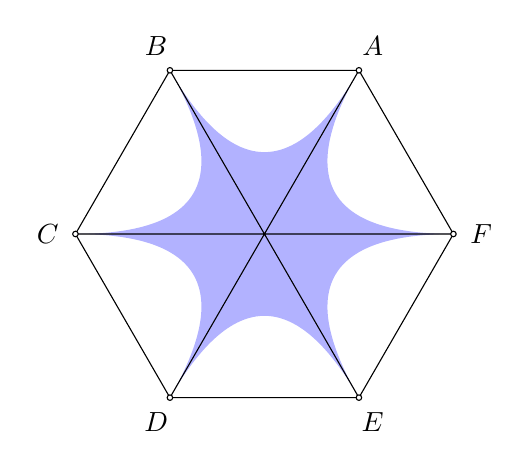
\begin{tikzpicture}[declare function={r=4;},x=.6cm,y=.6cm]
        \pgfmathsetmacro\a{2*sqrt(3)}
        \pgfmathsetmacro\b{\a-2}
        \path
        (0,0) coordinate (O)
        (60:r) coordinate (A)
        (120:r)  coordinate (B)
        (180:r) coordinate (C)
        (240:r) coordinate (D)
        (300:r) coordinate (E)
        (0:r) coordinate (F)
        ;
        \foreach \q in {0,60,120,180,240,300} 
        \fill[blue!30,smooth,rotate=\q] (O)--plot[domain=-2:2] (\x,{.25*sqrt(3)*(\x)^2+sqrt(3)})--(O);
        \draw (A)--(B)--(C)--(D)--(E)--(F)--cycle  (A)--(D) (B)--(E) (C)--(F);
        \foreach \x/\g in {A/60,B/120,C/180,D/240,E/300,F/0}\draw[fill=white] (\x) circle (1pt) +(\g:1em) node{$\x$};
    \end{tikzpicture}
}
    Hình phẳng $(H)$ được giới hạn bởi các parabol $(C_{1})$, $(C_{2})$, $(C_{3})$, $(C4)$, $(C_{5})$, $(C_{6})$ (phần tô đậm) là phần được dát vàng. Hỏi phần dát vàng này có diện tích bằng bao nhiêu centimet vuông {\itshape (không làm tròn kết quả các phép tính trung gian, chỉ làm tròn kết quả cuối cùng đến hàng phần chục)}?
    \shortans{13,9}
    \loigiai{
        Vẽ lại hình vẽ như sau gắn với hệ trục tọa độ $Oxy$:
        
        \centerline{
            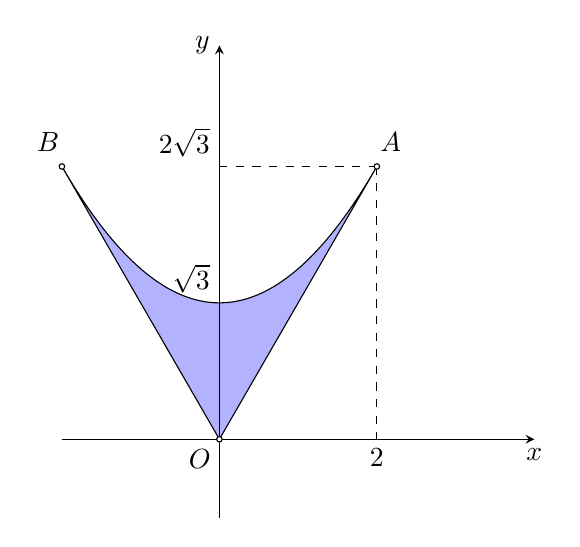
\begin{tikzpicture}
                \pgfmathsetmacro\a{2*sqrt(3)}
                \pgfmathsetmacro\b{\a-2}
                \path
                (0,0) coordinate (O)
                (60:4) coordinate (A)
                (120:4)  coordinate (B)
                ;
                \draw[fill=blue!30,smooth] (O)--plot[domain=-2:2] (\x,{.25*sqrt(3)*(\x)^2+sqrt(3)})--(O);
                \draw[-stealth] (-2,0)--(4,0) node[below]{$x$};
                \draw[-stealth] (0,-1)--(0,5) node[left]{$y$};
                \draw[dashed] (A)--(2,0) node[below]{2} (A)--(0,{2*sqrt(3)})node[above left]{$2\sqrt{3}$} (0,{sqrt(3)}) node[above left]{$\sqrt{3}$};
                \foreach \x/\g in {O/-135,A/60,B/120}\draw[fill=white] (\x) circle (1pt) +(\g:1em) node{$\x$};
            \end{tikzpicture}
        }
        
        Từ dữ kiện bài toán ta có tọa độ điểm $A(2;2\sqrt{3})$ nên đường thẳng $OA$ có phương trình $y=x\sqrt{3}$.
        
        Lại có parabol có dạng phương trình $f(x)=ax^{2}+b$ nên $f'(x)=2ax$. Do parabol tiếp xúc với $OA$ tại $A$ nên $f'(2)=\sqrt{3}$ và suy ra được $a=\frac{sqrt{3}}{4}$.
        
        Mặt khác parabol qua $A$ nên $f(2)=2\sqrt{3}$ suy ra $b=\sqrt{3}$.
        
        Như vậy parabol có phương trình $y=\frac{x^{2}\sqrt{3}}{4}+\sqrt{3}$.
        
        Diện tích hình phẳng giới hạn bởi đồ thị hàm số $y=\frac{x^{\sqrt{3}}}{4}+\sqrt{3}$; $y=x\sqrt{3}$; $x=0$; $x=2$ là 
        
        $S=\int\limits_{0}^{2}\left(\frac{x^{2}\sqrt{3}}{4}+\sqrt{3}-x\sqrt{3}\right)\dx=\left(\frac{x^{3}\sqrt{3}}{12}+x\sqrt{3}-\frac{x^{2}\sqrt{3}}{2}\right)\left|\begin{array}{l}2 \\ \\ 0\end{array}\right.=\frac{2\sqrt{3}}{3}$.
        
        Vậy diện tích cần tính $H=12S=8\sqrt{3}\simeq 13,9$  (cm$^{2}$).
    }
\end{ex}


\Closesolutionfile{ans}
